%!TEX root = ../thesis.tex

\chapter{Methodology and methods}
\label{chap:mm}

This first section of this chapter presents a description of the methodology of the planned dissertation work. This description is limited to matters relating to planning the execution of the work, without going into specifics about the methods themselves. The second section of the chapter presents an overview of the methods themselves, including information about how these plans evolved since the P2. This section also includes detailed accounts of the thought processes leading to the most important design choices. The rest of the chapter is devoted to a detailed account of the methods that underlie each of the processing steps in the final "proof-of-concept" software implementation, with accompanying flowcharts to illustrate the system design represented by the methods. A short section at the end of the chapter describes the implementation's software architecture, with explanation about certain technical design choices regarding the implementation.

\section{Methodological framework}
\label{sec:methodology}

This section contains a written account of the key stages into which the execution of this research can be divided. Each subsection describes one such stage, discussing the specific tasks performed during each stage as well as what has changed relative to my original plans. The methodology is also visually illustrated on a flowchart in Figure \ref{fig:methodologyflow}.

\subsection{Preparation}
\label{sub:preparation}

This project concerns a client - \ac{ndw} - with specific requirements and a pre-existing attempt at implementing a solution, in addition to aspects that are purely scientific. As a result, the first stage of the project involved \textit{consultation with the client} and with their commercial developers - \ac{rhdhv} - in addition to the task of \textit{familiarising myself with the research topic and literature}. The results of these preparation tasks were \textit{discussed internally} with my supervisors and used to \textit{define the final list of formal research questions} on the basis of focusing primarily on academic topics while also fulfilling the requirements of the client.

I executed this stage of the project according to my initial plans, little has changed during its realisation.

\subsection{Preliminary analysis, proposal writing}
\label{sub:preliminaryanalysis}

The second stage of the project involved \textit{further consultation with the client and their developers} to determine to what extent the commercial and scientific branches of the 3D-NDW project could be linked, and to allow me to understand the exact methods used in the prototype and the commercial implementation (which was being actively developed during this period of time). In parallel with these tasks, I \textit{performed the necessary in-depth literature review} and preliminary analysis. The preliminary analysis was comprised  of a \textit{close examination of the input datasets and their documentations} (input assessment), and based on this and the research questions, the \textit{final selection of relevant concepts and methods}. I also selected a range of illustrative geographical regions during the preliminary analysis, and cropped the datasets to their extents to \textit{create testing input files} for later development and testing. Lastly, the results of this stage were distilled to \textit{produce the project proposal}.

I executed this stage of the project according to my initial plans, but with a few small alterations. My initial plan was to put a slightly larger emphasis on performing preliminary analysis tasks, but the abundance of relevant literature and the complex task of creating a preliminary design for the methods (and the pipeline itself) limited the amount of time I could spend on it. I focused most of my effort at this stage in the research on the litrature review and the preliminary system design instead. This meant that during the next stage, I had a solid starting point in terms of background knowledge, and specific plans regarding what to start implementing.

\subsection{Analysis}
\label{sub:analysis}

The third stage of the research concerned carrying out most of the analysis. The period was characterised first and foremost by the intense development effort focused on the \textit{implementation of individual algorithms and steps of the workflow}. My original plan was to isolate this set of tasks and perform it separately from \textit{assembling the pipeline} from the individual modules. However, it proved to be more effective to develop the modules and incrementally extend the pipeline with them at the same time - an approach to which I switched after implementing the first few modules. This allowed me to resolve pipeline-level issues as part of the incremental refinement of methods, in addition to problems related to specific pipeline steps only.

Carrying out the \textit{accuracy-related analysis} was the last stage of the project that required active development on the program code. Testing the individual procedures and the pipeline was continuous during the implementation, with larger tests performed after reaching major milestones. Testing, and the assessment of performance and accuracy used the testing datasets I produced as part of the preliminary analysis. This was followed by a self-evaluation of the overall results of the research and a discussion of them with my supervisors, as well as a comparison of my results with those of the commercial project.

\subsection{Finalisation}
\label{sub:finalisation}

Both \textit{the implementation and the present report itself was improved and finalised} during this stage. The final version of the source code of this \LaTeX report and the implementation were published in their respective GitHub repositories. Furthermore, the outcome of the research and its findings relevant to improving the commercial implementation were communicated to and discussed with our client.

\begin{figure}
    \centering
    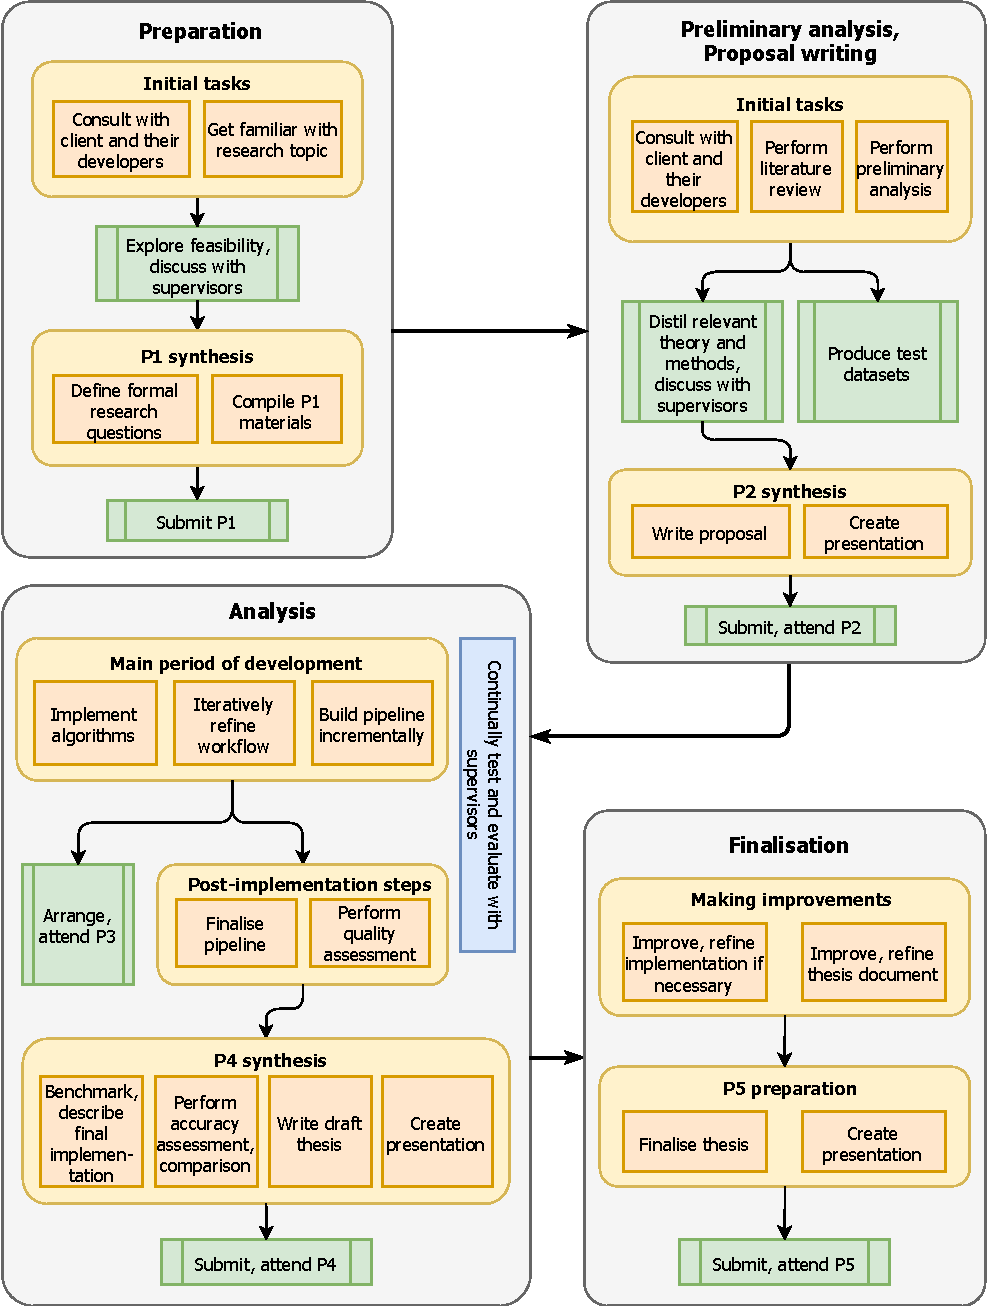
\includegraphics[width=\linewidth]{final_report/figs/methodology.pdf}
    \caption{Flowchart-style illustration of the top-level methodology of my dissertation research.}
    \label{fig:methodologyflow}
\end{figure}

\section{Overview of methods}
\label{sec:methodsoverview}

This section provides a structured overview of the steps of the processing pipeline. While the detailed descriptions in Section \ref{sec:methods} focus on explaining how exactly each step works, the purpose of the present section is to provide the rationale justifying their necessity and the reasons underlying certain major design choices, as well as to describe their role in the context of the system as a whole.

While the exact aims of the project materialised during the first two stages listed in Section \ref{sec:methodology} above, a brief description of the project existed before it. The project was originally conceived as a an academic continuation to the pre-existing attempt of \ac{ndw} to implement a solution to the 3D conversion of \ac{nwb}, re-using \ac{ndw}'s prototype implementation as the basis for a completed, academically sound version. During the aforementioned two stages, it became clear that \ac{ndw}'s pre-existing implementation is not robust and flexible enough to justify building the academic project on top of it. Hence, the entirety of the below pipeline was designed and implemented specifically for this academic project, no part of it represents code borrowed from the NWD prototype (or the RHDVH implementation).

\subsection{Proposed processing pipeline}
\label{sub:pipelineoverview}

The design of the pipeline is the result of a combined understanding of concepts described in related work, my own knowledge and experience relating to the geomatics discipline, as well as inspiration from the methods of the commercial implementation. The proposed workflow was built with a strong focus on finding answers to the research questions. Furthermore, it is also the result of a process of iterative refinement. In most cases, this only concerns the technical details of the algorithms implementing the pipeline steps, but in some cases I also made major changes to certain aspects of the general approach. Hence, in the structured overview below, I added a list item per pipeline step specifically to describe what changes, if any, were made to the given step.

As a brief summary of the general idea, the pipeline takes \ac{nwb}, decomposes it into roads whose surface can be modelled by 2.5D methods, and applies a set of mostly geomatics operations to produce the 2.5D road surface models that the elevations are then derived from to produce 3D-NWB. Accuracy-related considerations are not yet described in this section, these are first discussed in Section \ref{sub:accuracyoverview} below. A visual illustration of the main pipeline steps is shown in Figure \ref{fig:workflow}, showing only the titles of each workflow step in the order in which they are executed.

\begin{figure}[h]
    \centering
    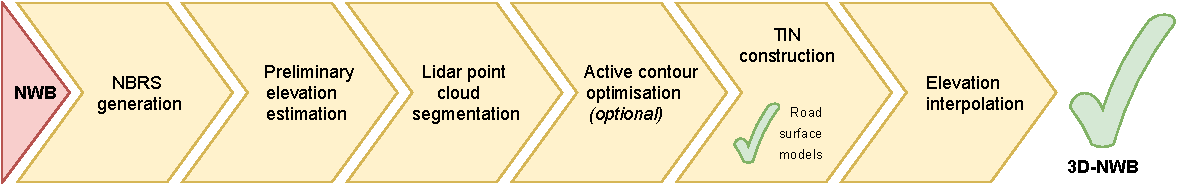
\includegraphics[width=\linewidth]{final_report/figs/workflow_steps.pdf}
    \caption{Illustration of the top-level steps and output of my processing pipeline.}
    \label{fig:workflow}
\end{figure}

\begin{enumerate}
    \item \textbf{Generating NBRS}
    \begin{enumerate}
        \item \textbf{Goal:} assemble optimal 2D profiles from the building blocks of \ac{nwb}.
        \item \textbf{Approach:}
        \begin{enumerate}
            \item Assemble \textit{non-branching road segments}, henceforth referred to as \ac{nbrs} (in both plural and singular) from \ac{nwb} geometry. To do so, look for series of \ac{nwb} \textit{wegvakken} (LineString objects) that represent the same road and join them into optimised 2D profiles - \ac{nbrs}.
            \item Perform the assembly of \ac{nbrs} in a way that maximises their length (optimal for lengthwise 2D operations such as polynomial fitting), minimising internal angles at the same time. Disallow self-intersection, so that each \ac{nbrs} can be modelled in 2.5D.
        \end{enumerate}
        \item \textbf{Purpose:} this step is necessary, because in addition to working with small-scale (short wavelength) features in the road network, we wish to be able to inspect trends that take place over longer distances in the network. The building blocks of \ac{nwb} (\textit{wegvakken}) can sometimes be short, occasionally only a few metres long. Hence, assembling them into \ac{nbrs} provides a better starting point for later steps.
        \item \textbf{Changes:} from the outset, I expected that simple methods based on progressing along 2D profiles, as well as modelling 2D profiles as a whole, would be useful for this project, and that a data structure serving this dual purpose would be necessary. Hence, \ac{nbrs} have always been part of my plans and their exact specifications did not change much during development.
    \end{enumerate}
    \item \textbf{Preliminary elevation estimation}
    \begin{enumerate}
        \item \textbf{Goal:} create a rough, preliminary 3D version of \ac{nwb}.
        \item \textbf{Approach:}
        \begin{enumerate}
            \item Based on the median elevation of nearby \ac{ahn3} points, associate \ac{nbrs} vertices with preliminary elevation approximates, thereby performing a crude 3D conversion of \ac{nwb}.
            \item Perform polynomial fitting on the 2D profiles that \ac{nbrs} represent. Identify vertices that are outliers with respect to the general shape of the \ac{nbrs} and interpolate values for them linearly.
        \end{enumerate}
        \item \textbf{Purpose:} this step is necessitated by the next one, point cloud segmentation. While it is possible to perform it without first performing a rough 3D conversion, I found it to be much more effective when the approximate 3D locations of \ac{nbrs} are already known by that point.
        \item \textbf{Changes:} this step represents and addition relative to the original plans. I started suspecting its benefits during the implementation stage, and subsequently added it to the pipeline design.
    \end{enumerate}
    \item \textbf{Point cloud segmentation}
    \begin{enumerate}
        \item \textbf{Goal:} create subclouds from the Lidar data containing points relevant to the roads represented by individual \ac{nbrs}.
        \item \textbf{Approach:}
        \begin{enumerate}
            \item Using their preliminary elevations, find "patches" of Lidar points in the 3D vicinity of \ac{nbrs} vertices. Progressing along the vertices of each \ac{nbrs} in a linear manner, fit planes on their Lidar patches. Where an unexpected change in the plane fits is detected, rely on points (vertices and densified vertices) extracted from \ac{dtb} to provide support.
            \item Where \ac{dtb} is also unavailable, accept the shifted (or missing) plane fits but perform a polynomial fit afterwards to identify planes that are unlikely to belong to the relevant road surface. Split the \ac{nbrs} into parts in such places, excluding the undesired regions from further consideration until the last pipeline step. 
            \item Based on the plane fits, decide which points in the patches are relevant to the road surface represented by a given \ac{nbrs}, and create subclouds by merging them (one for each \ac{nbrs} part). Include \ac{dtb} points that were used in places where \ac{ahn3} data was missing.
        \end{enumerate}
        \item \textbf{Purpose:} like \ac{nbrs} generation, this step also has a dual purpose. Firstly, it associates each \ac{nbrs} with a set of candidate Lidar and \ac{dtb} points that are likely to be relevant to them, thereby reducing the amount of Lidar points that will need to be processed later on. Secondly, it also excludes the majority of points which are close to a given road, but which were reflected from occluding geometry instead of its surface.
        \item \textbf{Changes:} originally, I only wished to detect where plane fits become inconsistent to exclude small-scale occlusion at this point. However, I eventually realised that by tracking changes in certain metrics, I could do so even in relatively long occluded regions. I then incorporated \ac{dtb} as a backup dataset to increase the reliability of this method, which made the solution work even where significant changes in elevation take place inside the occluded regions (such as in tunnels). I added the splitting of \ac{nbrs} into parts as a last tweak, after implementing the rest of the pipeline. This improved the results of later steps by removing areas without \ac{ahn3} \textit{and} \ac{dtb} coverage from the \ac{nbrs}.
    \end{enumerate}
    \item \textbf{Preliminary edge approximation}
    \begin{enumerate}
        \item \textbf{Goal:} create line geometries on both sides of \ac{nbrs} approximating the edges of the road surfaces.
        \item \textbf{Approach:}
        \begin{enumerate}
            \item construct cross-sections on \ac{nbrs} vertices and convert them to 2D elevation profiles by sampling \ac{ahn3} along their length. Perform linear regression on each, and select the outermost stable inlier points on both sides of the \ac{nbrs}. The two points are taken to represent the road edge locally.
            \item Assemble approximate road edges from the discrete edge points generated by the previous step, enforcing constraints regarding the expected shape of the road edges. Relax the constraints after a certain number of successive failures, to allow the algorithm to adapt to real-life changes in the road geometry.
        \end{enumerate}
        \item \textbf{Purpose:} the sole purpose of this step was going to be to provide edge estimates for active contour optimisation. After I made the decision to make active contour optimisation optional in the pipeline (due to its ineffectiveness), preliminary edges also became optionally needed for later steps, in place of the optimised contours.
        \item \textbf{Changes:} Due to the optional use of preliminary edges in \ac{tin} construction (in case optimisation is skipped), I needed to improve their quality significantly. This entailed the implementation of significant refinements to the underlying algorithm, as well as the constraints enforcement steps that I mentioned above.
    \end{enumerate}
    \item \textbf{Active contour optimisation \textit{(optional)}}
    \begin{enumerate}
        \item \textbf{Goal:} refine the preliminary edges based on road surface smoothness as described by Lidar.
        \item \textbf{Approach:}
        \begin{enumerate}
            \item Construct an attractor map from the subcloud of each \ac{nbrs} part, based on a scalar metric describing the local smoothness of the points.
            \item Use the preliminary edges and the attractor maps to perform active contour optimisation.
            \item Find a parametrisation for the active contour optimisation algorithm that works well with all testing datasets.
        \end{enumerate}
        \item \textbf{Purpose:} the original purpose of this step was to optimise the preliminary edges to the extent where they can be used to classify subcloud points either as surface or non-surface points. Since this was found not to work reliably, the current purpose of the step could be described as \textit{simplifying and enhancing the shapes of the preliminary edges}.
        \item \textbf{Changes:} even after improving all prior steps of the pipeline and sufficiently refining the parametrisation, the algorithm still produces mediocre results. As a result, I eventually implemented a bypass so that it can be skipped. Furthermore, I originally planned to apply morphological operations to attractor maps composited from maps generated using multiple different metrics. I found this to be ineffective in practice, the final implementation simply uses the raw results of the sole best-performing metric.
    \end{enumerate}
    \item \textbf{\ac{tin} construction}
    \begin{enumerate}
        \item \textbf{Goal:} model each \ac{nbrs} part by a \ac{tin} based on the subclouds and preliminary or optimised edges.
        \item \textbf{Approach:}
        \begin{enumerate}
            \item Seed each \ac{tin} by inserting points around the centre of the road unconditionally. Define the "centre of the road" based on the \textit{edges}, not the 2D location of the underlying \ac{nwb} centreline of the \ac{nbrs} part.
            \item Initialise each \ac{tin} by conditionally inserting points within the preliminary or optimised edges.
            \item Extend each \ac{tin} by conditionally inserting points further and further away from the centre of the road, beyond the edges if desired. 
        \end{enumerate}
        \item \textbf{Purpose:} this step also serves a dual purpose. On one hand, it satisfies our academic interest in creating 2.5D surface models of the roads. On the other hand, these models can then be used to interpolate final elevations for \ac{nwb} efficiently. Lastly, as the \ac{tin} consists of input elevation measurements, it allows output accuracy to be estimated in a straightforward manner.
        \item \textbf{Changes:} the original idea for this step was that the optimised road edges would be hard-coded in the \ac{tin} (a \ac{cdt} was planned), and only points within these constraint geometries would be inserted. Due to the ineffectiveness of active contour optimisation, I instead needed to create a \ac{tin} construction workflow that can make the best of the edges and subclouds \textit{without} making the assumption that the edges have near-perfect accuracy.
    \end{enumerate}
    \item \textbf{Elevation interpolation}
    \begin{enumerate}
        \item \textbf{Goal:} derive a final elevation for each \ac{nwb} vertex while enforcing continuity across intersections, and augment the original dataset with the results.
        \item \textbf{Approach:}
        \begin{enumerate}
            \item Interpolate in the respective \ac{tin}s to obtain a final elevation value for each vertex of each \ac{nbrs} part.
            \item At intersections, use the first elevation that was interpolated at that approximate 3D location and connect (snap) all other \ac{nbrs} to it that end or begin at that intersection.
            \item Use linear interpolation to fill in elevations in \ac{nbrs} where \ac{tin}-based interpolation was not possible.
            \item Mark the origin of each output elevation either as \ac{ahn3}, \ac{dtb} or linear interpolation.
        \end{enumerate}
        \item \textbf{Purpose:} obtain the final \ac{nwb} elevations and output 3D-NWB, keeping a record of which elevation comes from where.
        \item \textbf{Changes:} originally, I thought that enforcing continuity across intersections was going to be a bigger challenge. However, I found the \ac{tin} representations of the same intersections across different \ac{nbrs} to be consistent reliably, hence interpolating a single elevation (based on the first \ac{nbrs} part encountered) and snapping all subsequent ones to it works without issues in almost all scenarios examined.
    \end{enumerate}
\end{enumerate}

I was inspired by concepts and ideas from related work (see Chapter \ref{chap:rw}) while designing the original pipeline, and the final implementation retains many of these similarities. For instance, the point cloud segmentation step was inspired largely by \cite{oudeElberink_vosselman_2009} and \cite{boyko_funkhauser_2011}. The cross-section based edge detection workflow was inspired by curb detection-related work, such as \cite{yang_etal_2013} and the methods of the commercial implementation. The use of 2.5D-based modelling methods to represent surfaces extracted from the point cloud comes from \cite{oudeElberink_vosselman_2006}. The active contour-based workflow was inspired by \cite{boyko_funkhauser_2011} and \cite{gopfert_etal_2011}. In a way, my work can also be interpreted as a study of the effectiveness of relevant methods commonly found in the literature.

\subsection{Dependency of methods on specific datasets}
\label{sub:m_generalisation}

In this report I commonly refer to \ac{dtb} as a \textit{support dataset}. This is in part due to it always having been secondary to \ac{ahn3} because its spatial coverage is vastly inferior to \ac{ahn3} and it could not, by itself, fulfil the role \ac{ahn3} was given in this project, whch may therefore be called the \textit{primary dataset}. \ac{ahn3} contains enough data to make it possible to run the pipeline in the complete absence of \ac{dtb}. \ac{dtb} merely improves the results of the point segmentation step and extends the \ac{tin}s into areas not covered by \ac{ahn3} (preventing them from being split into parts in the process).

The reason why I often refer to the two elevation sources in such as way, is that it describes their \textit{roles} rather than their exact \textit{identity}. For the same reason, I also often refer to \ac{nwb} simply as the "road network". This is in line with my goal to make my methods as independent from the exact identity and properties of \ac{ahn3}, \ac{dtb} and \ac{nwb} as possible. Most parts of my methods should work regardless of the exact datasets used, as long as a few assumptions are satisfied. For instance, the primary Lidar dataset needs to be accurately classified, in particular vegetation should be clearly isolated from ground reflections. The assumptions regarding the primary dataset are detailed in Section \ref{sec:m_accuracyassessment}. \ac{dtb} could also be replaced with any generic dataset that contains accurate 3D geometries representing the surfaces of the relevant roads - or better still, with \ac{mls} data providing coverage where the primary \ac{als} one does not. The main difference is in scale between the primary and the support dataset; the purpose of the latter is to introduce data where the primary dataset has data \textit{gaps}. Recommendations regarding the support data are detailed in Section \ref{sub:improvementssupportdataset}.

The main concerns regarding generalisation (how well the methods and the implementation work independently from the properties of the datasets) are not related to the input datasets, but to the parametrisation of certain parts of the implementation. While many such parameters are exposed as arguments and can be customised by the user, there are also many that are hard-coded to avoid creating an API with an inconveniently long list of arguments. While the default parametrisation works in all the study areas of this project, there is no guarantee that they would always work equally well with other datasets - especially with ones containing road networks that possess different properties than that of The Netherlands (e.g. mountainous areas). However, being an open-source, proof-of-concept software, there is nothing to prevent potential reusers of my code from adapting it to their needs, including making changes to its fixed parametrisation.

\subsection{A note on DTB's role}
\label{sub:dtbrole}

In my P2 document, no specific mention was made about the role intended for \ac{dtb}, but a section was dedicated to speculating about potential uses. The evolution of its role in the final implementation was entirely up to the iterative refinement of the methods. In the end, the deciding factor in determining how \ac{dtb} could be used was that I found it to be useful for patching in gaps in \ac{ahn3} coverage, which is how the roles of primary and secondary dataset for \ac{ahn3} and \ac{dtb} came about.

Among potential uses I speculated about before starting the development was the use of \ac{dtb} as a means of contributing to edge estimation/optimisation, and to the lateral refinement of \ac{nwb} positions. However, I found \ac{dtb} road markings to be missing most commonly in the exact locations where they could have contributed to these aspects, for instance in sharp bends.

Using \ac{dtb} as a secondary dataset with the sole intention of characterising occluded road surfaces also generalises better, as the previous section makes clear. Consultations with \ac{ndw} also made it clear that they are in the position to commission the survey of additional georeferenced points or lines from Kragten (via a vehicle on which which commercial \ac{gnss} systems are mounted) or to purchase \ac{mls} data from Cyclomedia. Unlike \ac{dtb}, such data would \textit{not} correspond to specific road markings.

These circumstances are what prompted me to treat \ac{dtb} in a more generic manner, and to then extend this mindset to the way the rest of the datasets are used in my methods.

\subsection{Accuracy assessment of processing steps}
\label{sub:accuracyoverview}

As I emphasised in various places in this report already, it was among the aims of this research to perform the 3D conversion of \ac{nwb} in a way that output accuracy is as close the the input accuracy as possible, and that it can be evidenced and quantified either for the process as a whole, or for each output vertex individually.

As the literature review results in Chapter \ref{chap:rw} already indicated, there are various ways to go about this problem. The first and foremost decision one needs to make is whether an empirical or a theoretical approach is better suited to the given procedure. For our procedure, both appeared equally suitable at first. I first attempted an empirical approach, but having produced uncharacteristic results using this approach, I eventually settled on a combination of simple decision-making logic and a theoretical, mathematical framework. I will provide the details about the procedures later in this chapter, in Section \ref{sec:m_accuracyassessment}.

Below, I will outline the general approach, and the assumptions that are made when using it.

\subsubsection{Assumptions about influences}

My system design interpolates the output elevations from a \ac{tin} whose vertices are the Lidar road surface measurements themselves. I opted for this approach specifically because my literature review indicated that interpolating in such a \ac{dtm} appears to be the best option for large-scale terrain as well as in terms of accuracy, and because - assuming perfect ground filtering - it introduces no errors relative to the original Lidar data. However, as I explained in Section \ref{sec:lidaraccuracy}, the output accuracy in such a process is a factor of not only the generated \ac{dtm} and the interpolation technique used, but also of local, "environmental" factors. I made a range of assumptions regarding these influences before proceeding to the accuracy estimation step, which I will explain below.

The first factor to consider is the local \textit{accuracy of ground filtering}. In this project, most of the Lidar data was already ground filtered, as I made use of the excellent stock classifications that are present in \ac{ahn3} (please refer to Section \ref{sub:ahn} for more information on this topic). There is one exception to this rule: roads found on bridges are classified in \ac{ahn3} as bridges, including all objects on the roads such as guardrails and vehicles. Using the bridge classification also added objects over other roads (such as motorway signs), which locally violate the assumption that the road surfaces are ground-filtered.

However, processing steps in this research remove most non-road reflections from above road surfaces, and any remaining ones are eliminated by the careful conditional insertions of the \ac{tin} construction step. This holds both in theory and practice, as \ref{chap:r} explains. The number of outliers \textit{on road surfaces} is so small, that if we make the assumption that we only wish to interpolate elevations on road surfaces, we may regard the theoretical ground filtering effectiveness to be 100\%. As a result, the influence of non-road reflections (outliers on road surfaces) needs not be considered in the accuracy assessment.

The second factor to consider is the local sampling density of the Lidar points (and \ac{dtb}, where it was used in place of \ac{ahn3}). The assumption I made here is that as long as the \ac{tin} locally conforms with the theoretical minimum Lidar sampling density required to characterise a flat surface without oversampling it, the output accuracy will not suffer from any detrimental influence. I implemented simple logics to detect where interpolation has taken place in a location where the sampling density drops below this level. Vertices interpolated in such places do not receive an output accuracy value, and are thus flagged as having \textit{undetermined} accuracy. The details regarding the identification of a suitable local density threshold is found in Section \ref{sub:m_accuracypoorsampling} later in this chapter.

This second assumption holds, because in flat areas that are \textit{oversampled} by Lidar, literature indicates sampling density to have little to no correlation with empirically-derived error. In such areas, oversampling already occurs at point densities far lower than what is typical of \ac{ahn3}, apart from places where there are gaps in the data. Hence, a simple threshold-based evaluation can be deemed a sufficient measure to deal with the influence of this factor. This decision was made in view of the results of my empirical accuracy assessment results, which also indicated no correlation between sampling density and \ac{tin} model accuracy (see Section \ref{sub:accuracyempirical} for the details).

The last non-interpolation influence to consider is that, which is caused by terrain slope and ruggedness. Relevant literature discussed this topic also in the context of local sampling density, because it is especially in sparsely-sampled regions small, local variations that the ruggedness introduces may not be captured adequately. Road surfaces are, however, smooth. Furthermore, even inclined roads in our datasets are always characterised by smooth, gradual slope transitions - which makes sense, considering that both the motorways and municipal roads we are working with have high speed limits. The effects of local curvature on accuracy in this case may be neglected.

This combination of factors and assumptions lead me to implement an accuracy assessment workflow that either deems the accuracy to be undetermined (where sampling density is very low) or computes its accuracy solely based on the principles of error propagation through TIN-linear interpolation. This error propagation method predicts an \textit{increase} in the the standard error relative to that of the input for surfaces that are not very steeply inclined. The two categories also correspond with whether the output conforms with the requirements of the noise regulations or not. The details of this are found in \ref{sub:accuracyformal}.

\subsubsection{Influence of prior steps}

It may strike the reader as odd that it is almost only the last two pipeline steps that are discussed above in terms of what defines output accuracy. The reason behind this is that the \ac{tin}s are constructed entirely of \ac{ahn3} and \ac{dtb} points, thus making the standard vertical and horizontal error of each \ac{tin} node known. If the \ac{tin}s were constructed from points which were themselves "secondary information" (i.e. derived information) relative to the input, then the estimation of output accuracy would be more involved. However, this is not the case here - and therefore, wherever the above three assumptions hold, the quality of the \ac{tin} and the interpolation technique define the output accuracy alone.

The rest of the pipeline steps only affect whether the above assumptions are violated in a certain place or not. In particular, they may affect the local density of vertices in the \ac{tin}s and whether a \ac{tin} exists at the 2D location of a particular \ac{nwb} vertex or not. If we focus only on the influence of processing steps (i.e. we ignore the effects of physical factors and problems with the data), this may for instance be the result of a very poor polynomial fit in the preliminary elevation estimation step causing Lidar segmentation to fail locally, or the rare cases where preliminary edge estimation fails too many times in a row. Such blunders may cause issues in the \ac{tin}, but these too, will be picked up by the threshold-based evaluation and classified as unreliable accordingly.

Furthermore, we must also consider the fact that \ac{dtb} is densified prior to being converted to a pseudo-point-cloud. This is important because \ac{dtb}'s accuracy is defined in terms of its vertices, it does not apply directly to the line segments connecting them. For simplicity, I did not specifically consider how \ac{dtb}'s measurement error propagates to the densified vertices because if we considered such details regarding \ac{dtb}, then we would also need to consider its \textit{temporal} inaccuracy, which affects older \ac{dtb} geometry significantly. Since subsidence and potential other vertical land motions do not affect all areas uniformly, we cannot draw a simple relationship between the local age of the \ac{dtb} data and its accuracy without relying on relevant external data - such an analysis was not within the scope of this research. Furthermore, such an assessment may not apply to other support datasets. Instead, the assumption is made about the support data in general, that it possesses identical properties to that of \ac{ahn3}.

In another words, in this proof-of-concept implementation, \ac{dtb} merely \textit{simulates} a reliable support dataset, as \ac{dtb} itself does \textit{not} represent one. It is treated like an \ac{mls} dataset, and its accuracy is also evaluated on the same basis. Users specifically interested in the accuracy of the output when using \ac{dtb} should consider all output elevations marked as originating from \ac{dtb} data to be unreliable, and to certainly not confirm with the requirements of the noise regulations - even if the threshold-based evaluation does not indicate a missing accuracy value.

\subsubsection{Linear interpolation accuracy}

In areas with a complete lack of measurements, \ac{nwb} elevations are interpolated \textit{linearly} inside the \ac{nbrs}, based on the \ac{tin}-interpolated elevations that already exist by that point. This generally occurs under large occluding features (such as bridges), but also, less commonly, in the case of short road segments that are very poorly georeferenced in \ac{nwb}, as well as occasionally in places where large vehicles or dense vegetation resulted in smaller gaps of data in both \ac{ahn3} and \ac{dtb}. In more general terms, it occurs everywhere where it was not possible to interpolate a value in an underlying \ac{tin}, because none existed locally.

A typical, practical example is as follows: the Lidar segmentation workflow encounters a bridge with no \ac{ahn3} or \ac{dtb} coverage underneath. It splits the \ac{nbrs} into parts, one extending to the last \ac{nwb} vertex before the bridge, and the other starting at the first \ac{nwb} vertex after it. \ac{tin}s are constructed for the two \ac{nbrs} parts, but not in the space between them, i.e. underneath the bridge. The vertices in-between the two \ac{nbrs} parts (most likely 5-10 of them depending on the width of the bridge) will receive elevations that are linearly interpolated based on the closest elevations interpolated in the \ac{tin}s of the two \ac{nbrs} parts.

The output accuracy of these points is also not estimated. The primary reason for this decision is that the local sampling density is effectively zero. Since we do not estimate the accuracy in places with low sampling densities, it is well justified to also not do it where there sampling is even worse. In such places, formal accuracy can be safely assumed to be worse than that which is required by \ac{ndw} and the noise regulations.

To summarise, elevations marked as having been linearly interpolated always have undefined accuracy. However, undefined accuracy may also correspond to elevations that were interpolated from a \ac{tin}, but where the local \ac{tin} vertex density (Lidar sampling density) was too low to trust the value.

\section{Detailed methods}
\label{sec:methods}

Previous sections of this chapter described the methods underlying the pipeline steps in general terms. This section will go into more detail about the underlying processing algorithms. The level of detail will be greater than in previous sections, but not to the point where every step in the code is explained. Features of the implementation that are of a very technical nature are not included - the reader is referred to the open-source code and its documentation if they find themselves interested in learning about further details.

The focus of each subsection below is to explain, with the help of accurate flowcharts, how each pipeline step works, and to discuss major challenges encountered during development and how they affected the course of development. Most of these can be interpreted as further details about the top-level changes relative to the P2 plans that I already described in Section \ref{sub:pipelineoverview}.

\subsection{Splitting NWB into NBRS}
\label{sub:m_nbrsgeneration}

The first step of the pipeline is to create 2D profiles from the input road network with the properties mentioned in Section \ref{sub:pipelineoverview}, as this benefits various subsequent steps. The \ac{nbrs} are in practice made from a connected series of LineString objects from the road network in \ac{nwb} (i.e. they are \textit{assembled from the \textit{wegvakken}}). I implemented two algorithms based around the same general idea.

The first algorithm, which I call the "geometric algorithm", uses geometry only and thus generalises fairly easily; it could be used with any dataset comparable with \ac{nwb}. I call the second algorithm - which is an \textit{alternative} to the first - the "semantic algorithm", because it uses data from \ac{nwb}'s attribute table to try to assemble \ac{nbrs} in a way that only roads with identical roles (ramp, motorway lane, etc.) get added to the same \ac{nbrs}. This algorithm generalises less easily, but it demonstrates that the semantic information can provide important insights into network properties that would be difficult (even impossible) to recognise based solely on the geometry. Both algorithms are illustrated in Figure \ref{fig:nbrsgenerationflow}, and further textual descriptions are provided below. The results of the two algorithms are compared in Figure \ref{fig:nbrsgeneration0} in the Results chapter.

\begin{figure}
    \centering
    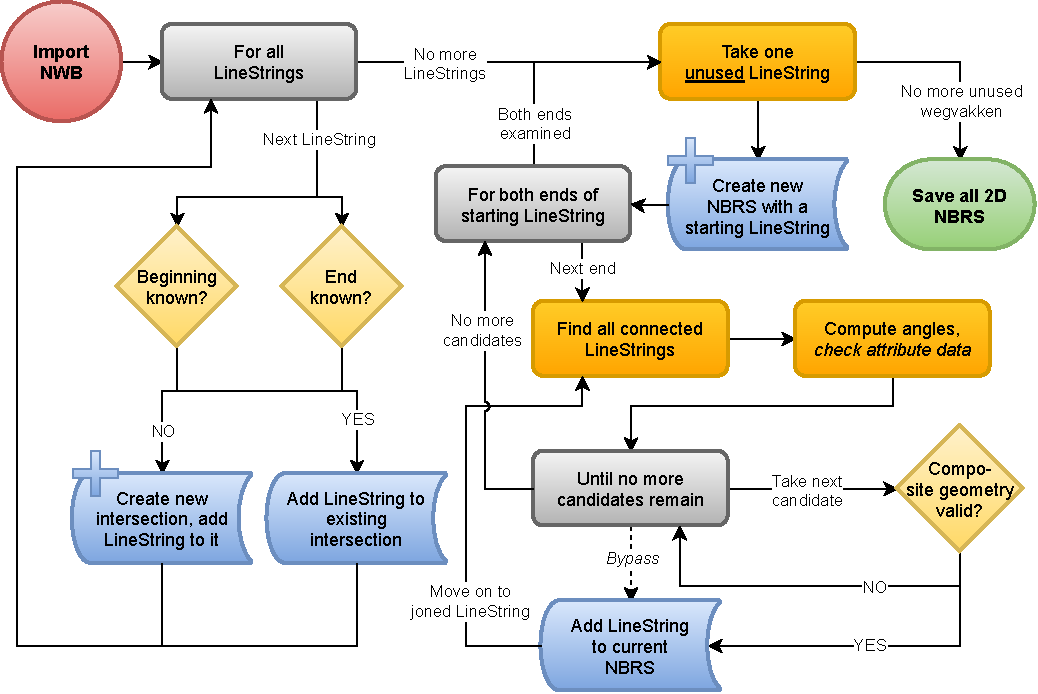
\includegraphics[width=\linewidth]{final_report/figs/nbrs_generation.pdf}
    \caption{Flowchart-style illustration of the \ac{nbrs} generation step of the pipeline.}
    \label{fig:nbrsgenerationflow}
\end{figure}

\subsubsection{Geometric algorithm}

This algorithm first creates a topological data structure from the input \textit{wegvakken}. Each \textit{wegvak} is a valid LineString, i.e. a connected series of line segments, which can be a few metres long or even hundreds of metres long. From here on in this section, I will consistently refer to \textit{wegvakken} as LineString objects to make the description more general. The topological data structure records which LineStrings of the road network start and end in which intersections. As this algorithm is not allowed to use the pre-made \ac{nwb} intersections from the attribute table, intersections are defined by their coordinates, rounded to one decimal. The topological data structure is based on hashing, hence it has good performance despite its reliance on coordinate-based lookup. The procedure consists of examining both ends of each input LineString and either creating a new intersection with it (if one does not exist at that location yet), or adding a reference to it in the intersection that is already found in the topological data structure. This is shown on the left in Figure \ref{fig:nbrsgenerationflow}.

The next step is to iteratively nucleate \ac{nbrs} generation until no unclassified LineString objects remain. The algorithm takes one LineString, initialises an \ac{nbrs} with it, and then attempts to extend it with further LineStrings on both ends. First, recursive extension is initiated on the last vertex of the LineString, and once that has completed, on its first vertex. The recursion examines the vertex, uses the topological data structure to find connected LineStrings and to connect one of them if certain conditions are met. Then, it progresses deeper into the recursion by doing the same with the LineString it just connected. The recursion ends, when no more suitable "extensions" can be found.

When the search for connected LineStrings succeeds in the above recursion, either a single one or multiple ones may be found. The latter corresponds to reaching a real-life intersection, in which case the algorithm needs to decide which one to connect based on a set of geometric conditions. First, the angles between the last line segment of the previous LineString and the first line segment of all the candidate LineStrings are examined, and the one with the angle corresponding to the straightest possible continuation of the road is selected. A composite geometry of the pre-existing \ac{nbrs} and the new segment is then created and tested for self-intersections. If the composite geometry fails this test, the next best candidate is examined, and so on until a candidate succeeds, or the iteration runs out of candidates - in which case none of the candidates are accepted and the recursion terminates. When both recursions (starting from the first and last vertices of the LineString that nucleated the \ac{nbrs}) have finished, the \ac{nbrs} is deemed complete and the next \ac{nbrs} is nucleated. The self-intersection test is also performed when only one connected LineString is found, i.e. not only when an intersection is encountered.

\subsubsection{Semantic algorithm}

The semantic algorithm is built on the same framework as the geometric one, as it is intended as a comparable alternative to the geometric one. Most steps of the procedure are slightly modified equivalents of the ones in the geometric algorithm, hence here I will focus on describing the differences.

The topological data structure of the semantic algorithm is based on the \ac{jte_id} records found in \ac{nwb}, which are unique identification codes belonging to each intersection of LineStrings in the dataset (including those of only \textit{two} LineStrings, i.e. not real intersections). Each LineString possesses an "end \ac{jte_id}" and a "beginning \ac{jte_id}" which are used to assemble the navigation structure in place of the coordinates in the geometric algorithm. The \ac{jte_id}s can be used to represent the topology of the dataset entirely, without any consideration for the geometry - indeed, it often describes topology more accurately than the geometry itself.

The nucleation of \ac{nbrs} takes place in a similar manner to the geometric approach, but here each \ac{nbrs} is associated with a specific wegnummer (road number) and BST code (a code related to the role of each road). LineStrings are only joined to an \ac{nbrs} if they have matching road numbers and BST codes, which is what the text \textit{check attribute data} in the flowchart refers to. The candidates are still processed in the order or decreasing angle optimality, like in the geometric algorithm. However, the composite geometries need not be checked for self-intersections, as roads satisfying the semantic conditions do not self-intersect in real life. This improves performance, as the intersection and validity checks of the resulting geometry is costly in terms of computational complexity. This shortcut is indicated by the dashed \textit{bypass} path in Figure \ref{fig:nbrsgenerationflow}.

\subsubsection{Challenges encountered}

I encountered three distinct issues while I was developing this part of the software. The first problem was that while \ac{nwb} has a near-perfect topological (graph) structure in its attribute table (represented by the \ac{jte_id}s), the same topology is not always represented by the geometry due to small-scale georeferencing issues. This means that the topology suggested by the geometry does not necessarily map to the \ac{jte_id}s exactly. In particular, LineStrings (\textit{wegvakken}) that are connected according to the attribute table may occasionally have disjoint or even overlapping geometries, which originally caused my software not to be able to merge them into the same \ac{nbrs}. Fortunately, once I started using the coordinate-based topological structure, I discovered that reducing the coordinate precision to only one decimal solved the issue in most places by effectively "snapping" the LineStrings together. However, this is not a full solution - \ac{nwb} georeferencing mistakes larger than 10 cm cannot be fixed this way.

A second issue was that the geometry of \textit{wegvakken} often \textit{reverses} in the middle of a connected series of LineStrings, requiring the implementation of a workaround in the code that computes the angles. The implementation now recognises where the geometry is stored in a reversed order relative to the \ac{jte_id}s and adjusts the angle computation accordingly. Lastly, for reasons related to external requirements that \ac{nwb} needs to meet, motorway ramps are connected to motorway lanes at unrealistic angles, occasionally causing the algorithm to merge ramps with motorway lanes and vice-versa. A dedicated workaround was also necessary here, to recognise this specific situation and to treat it correctly.

\subsection{Elevation estimation}
\label{sub:m_elevationestimation}

The elevation estimation stage of the pipeline consists of two operations. The first operation is to associate each \ac{nbrs} vertex with a preliminary elevation estimate based solely on nearby Lidar points, and the second a refinement step to eliminate occlusion-related artefacts. The procedure is illustrated by the flowchart in Figure \ref{fig:elevationestimationflow}.

\begin{figure}
    \centering
    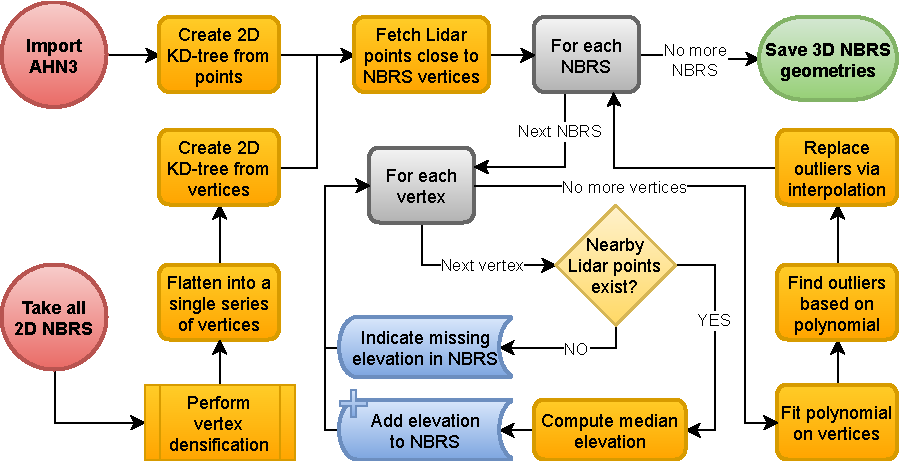
\includegraphics[width=0.9\linewidth]{final_report/figs/elevation_estimation.pdf}
    \caption{Flowchart-style illustration of the elevation estimation step of the pipeline.}
    \label{fig:elevationestimationflow}
\end{figure}

\subsubsection{Initial elevation estimation}

The process starts by importing \ac{ahn3}, from where elevations will primarily be derived. It is assumed that the input file is sufficiently small to allow in-memory use, i.e. that it is a cropped or clipped version of the full point cloud tile. Thus, this is the point in the procedure, where a global scaling solution would be most important. All other parts of the program work on the basis of processing subdivisions of the road network independently (\ac{nbrs} or the underlying LineStrings themselves), which is already a good starting point for scaling.

The imported point cloud is first converted into a 2D KD-tree, so that area-based queries can be performed efficiently on it. Then, points closer than a certain distance are fetched for each \ac{nbrs} vertex. The median elevation of the nearby Lidar points of each \ac{nbrs} vertex is then computed as a representative elevation estimate. Where too few points where found, the elevation is instead marked to be missing.

\subsubsection{Refining the preliminary elevations}

Following this step, each of the 3D-enriched \ac{nbrs} are fed into an outlier filtering algorithm. The algorithm generates a distance series based on the horizontal coordinates of the \ac{nbrs}, and fits a polynomial the corresponding elevation estimates. Since occlusion (due to overpasses or other objects) is almost always represented by short-wavelength data gaps or positive outliers in the Lidar data, these vertices are easy to isolate. The former is explicitly marked in the elevation series, while the latter show up as local clusters of large errors relative to the polynomial model. By interpolating values in such places, the quality of the preliminary elevations is improved considerably. The steps of this procedure are shown on the right in Figure \ref{fig:elevationestimationflow}. The resulting coordinates now represent 3D lines that preserve the input road network's 2D georeferencing, but which are enriched with elevations.

The replacement values are interpolated \textit{linearly} based on the series of inlier vertices, i.e. they are not determined by the polynomial fit. The reason for this is, that it is not always possible to find good fits using a fixed-degree polynomial, and while the polynomial model is always good enough to \textit{detect} outliers, its values are not conformant enough to \textit{replace} the original or missing elevations with.

This polynomial-fitting approach is reused in various subsequent parts of the implementation. It is similar to the approach in \cite{boyko_funkhauser_2011}, but it simplifies the global optimisation of splines into individual polynomial fits. Adapting the exact approach proposed in that research would certainly improve the effectiveness of my methods somewhat, but not drastically - I implemented subsequent steps in a way that they can deal with occasional mediocre-quality fits, and my results do not indicate that implementing a more sophisticated algorithm is justified.

\subsubsection{Vertex densification}

Although it is not strictly related to \ac{nbrs} generation, vertex densification is not listed as a discrete pipeline step as it is a rather trivial operation. It is only presented in this report as a pre-processing operation of preliminary elevation estimation. It is shown in \ref{fig:elevationestimationflow} as the first processing step that acts on 2D \ac{nbrs}.

Vertex densification of the \ac{nbrs} vertices refers to the operation of taking the LineStrings that make up each \ac{nbrs}, and adding vertices to their line segments until no distance between the vertices is bigger than a certain threshold. In my implemetation, this takes place as a recursive iteration. Each LineString of each \ac{nbrs} is considered, and the densification algorithm is called on each line segment. The recursion consists of breaking the line segment in two halves if it does not comply with the threshold (a vertex is added in the middle), and then proceeding deeper into the recursion by doing the same with the two resulting halves. The densified geometries are assembled when returning from the frames opened by the recursion.

Like \ac{nbrs} generation, vertex densification is done for the benefit of subsequent operations. Many operations - such as the present step - act on each vertex separately, gathering information related to the vertex from its \ac{ahn3} and \ac{dtb} neighbourhood. Since the posting distance of \ac{ahn3} is several magnitudes smaller than the line segments of \ac{nwb} LineStrings, increasing the density of \ac{nwb}'s vertices has practical benefits. It not only increases the resolution at which elevation can be sampled, but it also means that large-scale trends in the data will be represented more dominantly, i.e. algorithms will be better able to tell which parts of the road represent the road surface, and which ones are outliers due to occlusion. The practical benefits of this step were observed during development, and vertex densification was made an intrinsic part of various other parts of the pipeline too.

\subsubsection{Challenges encountered}

The main challenge encountered was related to the random reversals of LineStrings (\textit{wegvakken}) that I already mentioned in Section \ref{sub:m_nbrsgeneration}. At this point, I needed to implement a workaround that flips reversed \textit{wegvakken} into the correct orientation before moving on to the polynomial fitting step. In fact, it is the polynomial fitting step that had first drawn my attention to this problem, as it was impossible to get it to work before realising that parts of the 2D profiles contained vertices in the wrong order. The rectification of the orientation of the geometries takes place relative to the first LineString in the \ac{nbrs}. These are then rotated back into their original orientations after the refinement step, to avoid introducing changes to the 2D geometry of \ac{nwb}.

A second challenge was to find a good benchmark of what to consider outliers after fitting polynomials. I needed to choose a metric that works well with all the types of typical occlusion-related artefacts that show up in the data, such as overlying bridges of various heights, civil engineering structures of such bridges next to and above roads, motorway signs, tunnels, and so on. After experimenting with various approaches, I settled on one that involves setting the threshold dynamically, as a multiple of the standard deviation of the residuals between the initial elevation estimates and the polynomial-based elevations. Where the standard deviation is smaller than a certain threshold, I artificially raise it to a preset minimum to avoid performing linear interpolation where the conformance is very good.

\subsection{Lidar segmentation}
\label{sub:m_lidarsegmentation}

The Lidar segmentation step is more complex than the previous two, and some of the intricacies are omitted in the relevant flowchart (Figure \ref{fig:lidarsegmentationflow}) to keep its complexity manageable. I will attempt to fill in some of these details here in the text, referencing where approximately in the flowchart they occur. The goal of this step is to create subclouds from the Lidar data containing points relevant to the roads represented by individual \ac{nbrs}.

\begin{figure}
    \centering
    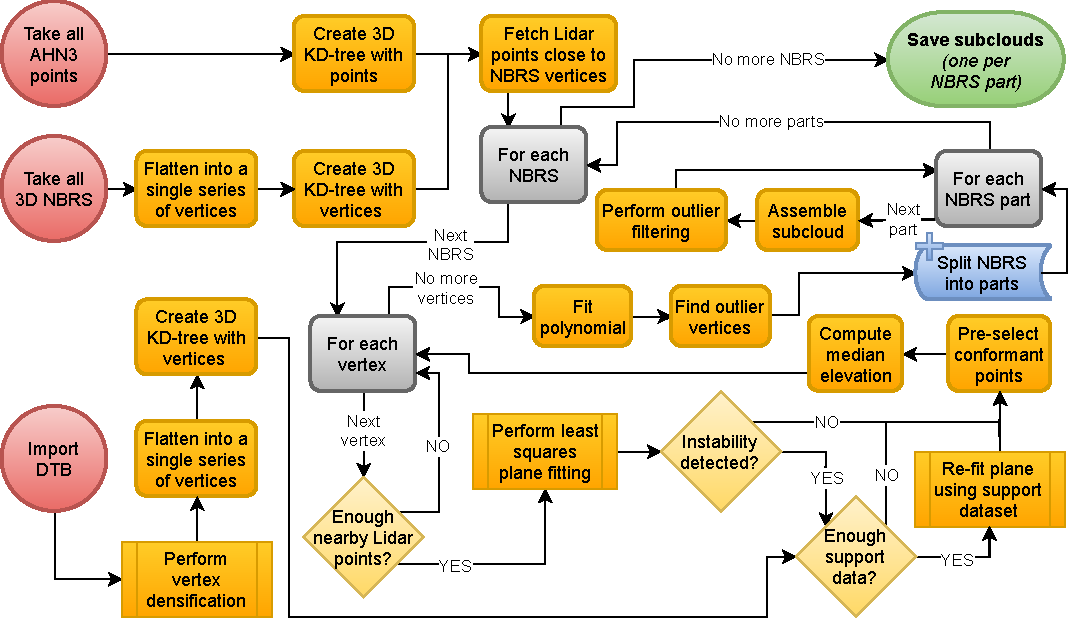
\includegraphics[width=\linewidth]{final_report/figs/lidar_segmentation.pdf}
    \caption{Flowchart-style illustration of the Lidar segmentation step of the pipeline.}
    \label{fig:lidarsegmentationflow}
\end{figure}

\subsubsection{Preparation and plane fitting}

The program first creates KD-trees from the 3D point cloud, all 3D \ac{nbrs} vertices, as well as all vertices found in the support dataset, \ac{dtb}. The lines in \ac{dtb} are also vertex-densified prior to being converted into a point cloud and then into a KD-tree. The densification drastically increases the effectiveness of using \ac{dtb} as a point cloud. The reason why \ac{dtb} is treated like a point cloud was discussed in Sections \ref{sub:m_generalisation} and \ref{sub:dtbrole}.

Much like in the preliminary elevation estimation workflow, a Lidar point cloud KD-tree query is performed as a bulk operation on each \ac{nbrs} vertex (using the KD-tree made from the \ac{nbrs} vertices). This results in a "patch" of Lidar points being selected for each \ac{nbrs} vertex. Here, the underlying selection geometry is a sphere, rather than a 2D circle (as was the case in preliminary elevation estimation). This means that the relevance of the selected points will already be far more certain than before.

Each of these patches are further processed to enhance the results. The program fits a plane on each patch of Lidar points using the \ac{mle}. Planes are only fitted if there are a set minimum number of points to support it, a threshold which is defined in terms of reaching a certain minimum point density inside the patch. If it is not reached, the points may still be passed on if a lower threshold is reached, in the hope that the support dataset (\ac{dtb}) can re-position the plane to them in later stages of the algorithm and find some of them to be conformant with it. Below this second threshold, neither a fitted plane, nor the points are passed on. In the flowchart (Figure \ref{fig:lidarsegmentationflow}), this stage is shown in a simplified form which excludes the logical branch between the two thresholds.

\subsubsection{Refining plane fits and pre-selecting points}

Next, the program considers the vertices of each \ac{nbrs} one by one, in the order in which the vertices geometrically represent a valid road centreline. The program searches procedurally for places where the succession of fitted planes may indicate a break in shape of the surface. At the beginning of the iteration, the program initialises three variables describing the \textit{previous} plane fit's relative position to the 3D \ac{nbrs} centreline, the median elevation of the relevant patch's Lidar points, and the standard deviation of their distances to the fitted plane. By examining variations in these metrics, the algorithm can detect where the plane fits become unstable. It always compares the values of the current iteration to the ones from the previous iteration. Significant changes relative to the previous vertex and plane may indicate the presence objects occluding the sensor's view of the road's surface. I determined the exact metrics and parameters (thresholds) to detect "plane instability" based on experimentation and iterative refinement. The current setup works well with all testing datasets examined. This step is represented in the flowchart by the conditional element labelled \textit{"Instability detected?"}.

Originally, the algorithm was configured to automatically revert to the previous plane in case of plane instability and be allowed to use the reverted plane for a few iterations before asking help from the support dataset, in case the road emerged from underneath the occluding object after a few iterations at roughly the same elevation at which it disappeared. If the support dataset could also not help (due to e.g. a lack of coverage) after the expiration of the tolerance period, the algorithm would "give up" and move on to the next \ac{nbrs}. This meant that long occluding objects and no \ac{dtb} coverage could prevent the algorithm from processing certain \ac{nbrs}, for instance ones containing tunnels.

\subsubsection{Handling breaks in the trend and missing data}

I eventually revised this algorithm to be more robust and to produce useful results even in a complete absence of a support dataset such as \ac{dtb}, wherever there is \ac{ahn3} coverage. In the current version of the implementation, the algorithm is only allowed to attempt to use the previous plane \textit{once} before trying to use \ac{dtb}. The point cloud generated from \ac{dtb} contains road surface measurements only, so it can be relied on to provide "assistance" where \ac{ahn3} is ambiguous.

If a previous valid plane exists, then \ac{dtb} is queried for points relatively close to it. If not, then the centre of the query becomes the current \ac{nbrs} vertex itself. If a reasonable number of \ac{dtb} points could thus be recovered, then the process is repeated by performing a second KD-tree query on the centroid of these \ac{dtb} points, and the plane is then re-fitted onto the retuned points. This second query ensures that as many useful \ac{dtb} points are included as possible. The program then assesses the distribution of \ac{ahn3} Lidar points in the patch close to the re-fitted plane, and if the majority are found to be conformant with it, then the plane is re-fitted a third time to make sure that in the end it is based on the Lidar points and not the support data wherever possible. The necessity of this last step is related to the temporal problems with \ac{dtb} already mentioned in Section \ref{sub:dtb}.

In the new version of the algorithm, the program does not declare failure if it is no longer allowed to revert the current plane to the previous one, and also finds support data to be unreliable or missing. Instead, it simply relaxes its conditions and continues as though it were starting to process anew (i.e. as if it were initialising a \textit{new} \ac{nbrs}). This bypass allows the program to continue the procedure even if it is aware that there was a noticeable shift in the position of the fitted planes, or a gap in \ac{ahn3} coverage. These areas are now handled separately, outside of this iteration.

Each successful iteration of this algorithm finishes by pre-selecting those \ac{ahn3} and \ac{dtb} points which conform well with the final plane fit, and saves them as individual patches. The median elevation of the pre-selected points is saved, as it will be used in the next step.

The above iteration is shown as the loop labelled \textit{"For each \ac{nbrs} vertex"} in Figure \ref{fig:lidarsegmentationflow}. In the implementation, the nesting of the iterations in different, but this description is easier to understand and is fully equivalent to the implemented version in terms of what it achieves. The same is true about the top-level iteration (\textit{"For each \ac{nbrs}"} in the flowchart), which in the implementation is broken into several parts for programming convenience.

\subsubsection{Breaking NBRS into parts}

After the above iteration, a post-processing procedure is executed before moving on to the next \ac{nbrs}. Based on the median elevations of the patches saved during the iteration, the program once again has a new 2D profile which it can examine for outliers. Missing elevations in the series are indicative of a lack of coverage in both \ac{ahn3} and \ac{dtb}. Outlier elevations indicate that the corresponding plane fit was corrupted by occluding features that caused occlusion or partial occlusion, and that it was also not possible to rectify the plane fit based on \ac{dtb}.

The program generates a boolean mask of where either of these issues are present in the elevation series. This is used to construct a list of intervals inside the \ac{nbrs} that were found to be affected by neither of the above two problems. Through this, a further subdivision of the road network is introduced: \textit{\ac{nbrs} parts}. Each part corresponds to an interval in its parent \ac{nbrs} with reliable combined \ac{ahn3} and \ac{dtb} coverage. Before splitting the \ac{nbrs} in such a way, the boolean mask is post-processed to eliminate references to artefact affecting a few vertices only. Removing references to such small problems ensures that \ac{nbrs} do not get split into too many parts. Unlike larger data gaps or zones of occlusion, such small ones do not affect the quality of the results of subsequent steps.

The patches of \ac{ahn3} and \ac{dtb} points are then combined into a subcloud, one for each \ac{nbrs} part, making sure not to add duplicate points (the same point may be part of multiple patches). A quick outlier filtering step is applied to them, to eliminate points which are isolated (have no neighbours within a certain distance). This is easy and computationally efficient to execute by converting the data into KD-trees and performing nearest-neighbour queries on them.

A hashed structure is initialised at this point in the program that allows the program to remember which points in the subclouds originated from the support dataset. The use of this structure is described in Section \ref{sub:m_interpolation}.

\subsubsection{Challenges encountered}

The above description already contains mentions of how my methods relating to treating breaks in the trend and missing data evolved. Here, I will further elaborate on this topic.

The simple approach of starting on one end of the \ac{nbrs} and examining its vertices one by one turned out to have significant limitations when I began to debug my implementation with the testing datasets. As it has no concept of global trends in the \ac{nbrs}, it can only rely on its previous iterations to detect breaks in the trend and to make decisions based on it. Because of this, in regions with occlusion-related or missing \ac{ahn3} data \textit{and} missing \ac{dtb} coverage, significant problems could arise.

The original algorithm was able to detect where a data gap with or without occlusion-related data would occur, but it was not always capable of continuing on the other side of the problematic area. Projecting the last "trusted" plane to the other side would not work, because even a small erratic tilt in the plane would become a large enough problem by the time the algorithm reached the other side of the problematic region, that all the valid road surface points would be found non-conformant. Furthermore, even if a perfect plane fit existed before the problematic area, if the elevation of the road changed by the time it emerged on the other side of it (e.g. on the opposite side of a long tunnel), the method would still fail.

Eventually, I realised that moving part of the decision-making mechanism outside of the iteration would solve these issues. I transitioned to first saving Lidar patches per vertex separately (instead of adding them straight to a subcloud), constructing a polynomial based on their centroids to describe the overall trend, and detecting and excluding patches with unrelated points this way.

A second revision to the algorithm was necessary after the implementation of the next three pipeline steps. Keeping regions with no coverage inside \ac{nbrs} meant that in subsequent steps, I was optimising contours and continuing road surface models across them as well - sometimes over hundreds of metres or more. This turned out to be problematic especially with active contour optimisation, which frequently ended up producing corrupted outputs as a result. This is the issue that splitting \ac{nbrs} into parts solves. Regions that lack any elevation measurements do not become part of any of the \ac{nbrs} parts, and as a result, later steps of the pipeline do not need to handle them. They are only considered again at the very last step of the pipeline, described in Section \ref{sub:m_interpolation}.

\subsection{Edge approximation}
\label{sub:m_edgeapproximation}

The generation of preliminary edges is based on approximating the location of the two road edges at road centreline vertices. For each \ac{nbrs} part, the two road edge lines are assembled from these discrete edge point estimates. The process is illustrated in Figure \ref{fig:edgeapproximationflow}.

\begin{figure}
    \centering
    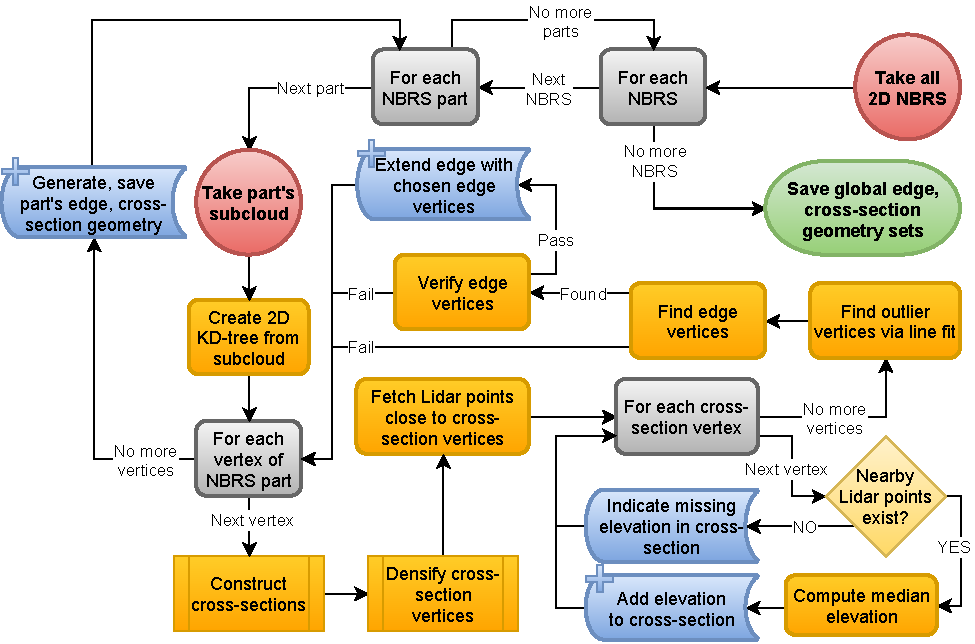
\includegraphics[width=\linewidth]{final_report/figs/edge_estimation.pdf}
    \caption{Flowchart-style illustration of the edge approximation step of the pipeline.}
    \label{fig:edgeapproximationflow}
\end{figure}

\subsubsection{Constructing edge point candidates}

First, the subcloud of each \ac{nbrs} part is used to create a 2D KD-tree. 2D suffices here, because it is a reasonable assumption to make at this point that the subclouds of \ac{nbrs} parts no longer have a significant number of points that violate the 2.5D assumption (e.g. reflections from occluding objects). On each vertex of each \ac{nbrs} part, a cross-section is then constructed. Cross-sections are line segments roughly orthogonal to the centreline locally. Their azimuths are based on the mean azimuths of the two line segments that contain the given vertex, except for the first and last vertices, which are simply based on their single parent segment's azimuth. The cross-sections are vertex-densified, and their densified vertices are used in a bulk KD-tree query. Lidar points close to cross-section vertex are thus identified, and the median elevation of each group is saved as the elevation of the given vertex. This step works on a small, sub-metre scale, meaning that using the native density of \ac{ahn3} (no thinning applied) is particularly important from here on.

Each cross-section then represents a 2D elevation profile, with the corresponding centreline vertex in the middle. A line fit for the 2D profiles of each cross-section is computed and outlier vertices are identified based on them. The program then tries to find suitable edge points among the inlier cross-section vertices on both sides of the centreline, in each cross-section. Together, these points will form the preliminary edges. In each of the cross-sections, the program starts from the outermost cross-section vertex and progresses inwards. Once a certain consecutive number of inliers is encountered (with no outliers in-between them), the program assumes having reached the road surface and flags the current vertex as the edge vertex.

The total length of the cross-sections, which is a constant parameter, represents the maximum road width the program can work with. The optimal value of this parameter depends on the possible road dimensions in the given road network. If too small a value is used, the preliminary edges may lie too far inwards from the real-life edges, thereby excluding large parts of the real-life road surface as a result. If it is too large however, false positive hits outside the real-life road surface will corrupt the preliminary edges, especially where roads are thin and other smooth surfaces are found in their surroundings.

\subsubsection{Enforcing constraints}

Flagged vertices are only accepted as edge vertices if they also pass a range of further conditions relating to a minimum road width, as well as sudden elevation changes and road width changes. The minimum road width is enforced for each pair of edge points individually. However, much like in the first part of the Lidar segmentation step, the latter two conditions are evaluated on the basis of comparing the metrics of the current edge point candidates to a mean value from a set number of previous iterations. Only if this verification procedure succeeds, does the program extend the \ac{nbrs} part's preliminary edges with the new vertices.

In areas where the above procedure fails multiple times consecutively, "gaps" are created in the preliminary edges. These are not real gaps in the sense that the last pair of edge points before the gap, and the first pair after, are still connected in the output - it simply means that there are no edge vertices locally. Compared to the artefacts that would appear in the absence of the above threshold enforcement procedure, creating small gaps is an acceptable compromise, especially if the \ac{nbrs} were sufficiently vertex-densified prior to this step.

However, long gaps may cause various problems in later pipeline steps. To avoid creating them, a relaxation of the conditions takes place after a set number of failures. After relaxing the conditions, the first inlier point on both sides is selected when fitting the next cross-section with a line, and the constraint regarding sudden changes in width is also ignored. Immediately after a success, the constraints are re-enabled. This temporary relaxation allows the algorithm to regain its references even if a sudden real-life change in the road's dimensions is encountered. It also helps in scenarios where the location of the edge is ambiguous.

Lastly, once per \ac{nbrs} part the program generates the final 3D cross-section and edge geometries and saves them. After all \ac{nbrs} parts have been processed, the global cross-section and preliminary edge object is also created.

\subsubsection{Challenges encountered}

Originally, this step was going to be a preparatory step for the sole purpose of providing initial edge shapes for the active contour optimisation algorithm. I first implemented it almost exactly to the specifications found in the P2 document. However, it soon became clear that better active contour optimisation results require better preliminary edge estimates, and thus I had to implement a range of tweaks and improvements in an iterative manner. It seemed that the best active contour optimisation results corresponded to where the preliminary edges were on the road surface, slightly inwards from the location of the real-life road edges. This is why the algorithm starts from the outer edges of the cross-sections, and progresses inwards until it can safely conclude that is has already been inside the road surface for at least a few vertices.

A further challenge corresponded to the point in development when I decided to make active contour optimisation optional. I needed to implement modifications to these methods to allow preliminary edges to be used for \ac{tin} construction directly, at the same time maintaining compatibility with active contour optimisation. This is what resulted in the addition of the system of constraint enforcement and constraint relaxation that takes place right before accepting a pair of edge point candidates. The main reason why this is beneficial for \ac{tin} construction is that it ensures that the edges cannot shrink too much, while also reducing the chances of road widths being overestimated due to small-scale issues.

The former ensures that road centrelines are found between the preliminary edges under normal circumstances, and with enough distance between them and the edges to ensure that Lidar points will found there during the \ac{tin} initialisation step. Without this, it may be possible in certain exceptional cases, that the \ac{tin} would not exist at the 2D position of the \ac{nwb} vertices and we would therefore not be able to interpolate an elevation for \ac{nwb} there. The latter (maximum road width) decreases the chances of including off-road points in the road surface models, both during \ac{tin} initialisation and extension. For more information about the \ac{tin} construction step, please refer to Section \ref{sub:m_tinconstruction}.

\subsection{Active contour optimisation}
\label{sub:m_activecontours}

The optimisation of preliminary edges is based on generating one attractor map for each \ac{nbrs} part based on subcloud point normals, and running active contour optimisation to attract the preliminary edges to certain features in the attractor maps. The procedure is illustrated in Figure \ref{fig:edgeoptimisationflow}.

\begin{figure}
    \centering
    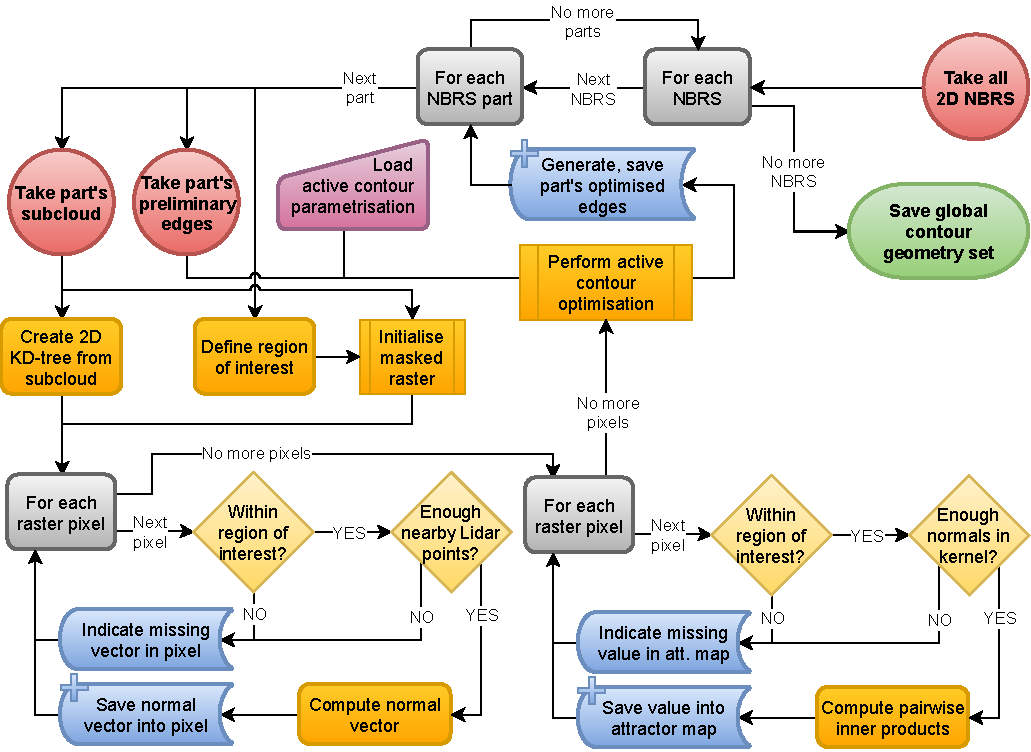
\includegraphics[width=\linewidth]{final_report/figs/edge_optimisation.pdf}
    \caption{Flowchart-style illustration of the active contour optimisation step of the pipeline.}
    \label{fig:edgeoptimisationflow}
\end{figure}

\subsubsection{Attractor map generation}

The procedure underlying this step is once again based on a 2D KD-tree of the subcloud of the \ac{nbrs} part. 2D suffices because attractor maps are 2D rasters, and once again, because we are safe to assume at this point that the subclouds of \ac{nbrs} parts mostly describe 2.5D surfaces. The rasters are first georeferenced in the same coordinate system as the rest of the data, after they are initialised. For each of them, a region of interest is derived by buffering the appropriate centreline by a certain amount. The rectangle-shaped raster is then masked out everywhere except for pixels whose centres lie within the geographical region delineated by the buffer polygon.

The centre of each unmasked pixel is then used in a bulk KD-tree query to find a small patch of nearby Lidar points for each. For pixel centres that have a sufficient number of neighbouring Lidar points, a normal vector is computed. These normal vectors are computed as the normal vectors of the local plane fits of each such patch of Lidar points, and the \ac{mle}-based approach is re-used in my implementation (originally written for the Lidar segmentation step).

Normal vectors can be stored in the pixels in my framework, but they cannot be used directly in active contour optimisation because it requires scalar pixel values. To derive scalar values from the vectors, I designed a kernel-based approach. The pairwise inner products of the normal vectors of pixels falling into the moving window are computed, and the median of the value is saved. Since computing inner products is computationally expensive, not all pairwise combinations of the normal vectors in the kernel are dotted, only a representative random subset.

\subsubsection{Running the optimisation algorithm}

From here on, all operations take place in a temporary coordinate system which is defined simply in terms of the number of pixels in the X and Y dimensions from the top left corner. Before the preliminary edges can be overlain on the attractor map, they each need to be transformed into this coordinate system via an affine transformation. Together with the attractor maps and a suitable parametrisation, the preliminary edges are now ready to be optimised. The optimisation algorithm is run separately for the edges on the two sides of the centreline, and the output optimised edges are then assembled into a single polygon.

The scikit-image implementation of active contour optimisation is based on the original paper in which this procedure was first described scientifically: \cite{kass_etal_1988}. In addition to taking the attractor maps and the preliminary contours as input, it also takes a set of parameters that can be tweaked to manipulate aspects of the optimisation. The most important aspects for us in this project are contour smoothness, attraction to brightness or darkness, attraction to edges and the total number of allowed iterations. In Section \ref{sub:r_activecontours} I describe the final configuration of values for these parameters.

\subsubsection{Challenges encountered}

In terms of the first version of my implementation, the main challenge here was the trial-and-error nature of getting active contour optimisation to perform acceptably for the wide variety of road geometries and attractor map features that are possible in our datasets. I needed to refine the parametrisation to work well with the input data, but since I was also producing the input data myself, I was also in the position to fine-tune that in turn. As a result, the task was a joint refinement procedure involving all prior steps in the pipeline leading up to this point, in addition to just adjusting the parameters.

Of all the aspects of the input data that I tried to optimise, I invested the greatest amount of effort in trying to pre-process the attractor maps to enhance their compatibility with contour optimisation. I tried various moving-window techniques such as many types of edge detection, edge enhancement, blurring, as well as morphological operations such as dilation, erosion, opening, closing, and many combinations thereof. I also tried compositing the resulting rasters. Sadly, I eventually concluded that none of these operations can achieve a noticeable improvement in the results, with the original kernel-based normal vector attractor maps and the native edge detection of active contour optimisation still producing the best results after several days spent on this.

Making matters worse, I found active contour optimisation to work only at high raster resolutions, with a pixel size around 0.5 metre typically producing the best results overall. Unfortunately, computational complexity grows non-linearly with decreasing pixel size, making debugging and fine-tuning very difficult, as well as putting the usefulness of such an algorithm into question considering the scale of the input data.

A further problem I found is that there are occasional small-scale features in the input data that tend to confuse active contour optimisation. Even for relatively short iteration lengths, such small artefacts may unpredictably corrupt entire \ac{nbrs} part contours. For instance, small Lidar gaps due to stationary vehicles frequently overlap with the region where the road edges are suspected to be found. Active contour optimisation has no concept of no-data pixels, and reacts unpredictably to these holes regardless of what one uses as filling values. Another similar issue is that road edges are often characterised by sudden slopes beyond their edges, but with further flat regions beyond them. This often creates a second contrast in brightness that active contour optimisation may confuse with the real road edge. Features such as these frequently draw the contours further from the road than what would be acceptable to accurately classify Lidar points within the contours as road reflections.

Lastly, the effectiveness of the method is also far too reliant on the accuracy of the preliminary edges. The algorithm is sensitive to even the smallest of blunders in preliminary edge detection, and is also prone to fail in no-data regions. After I implemented the code to split \ac{nbrs} internally into parts where longer regions suffer from the absence of data, part of this issue was solved, but another remained: where \ac{dtb} is available but not \ac{ahn3}, preliminary edges tend to shrink significantly, which often corrupts the optimised edges.

While the method works and produces usable results, the poor quality of the output and its unreliability in general prompted me to make it possible to bypass its use in the software. This required modifications to various previous steps of the pipeline, as well as all subsequent ones - a significant challenge. This bypass in turn puts into question the relevance of much of the pipeline structure, many parts of which were intended to lay the groundwork for active contour optimisation, and to make use of its output. I elaborate on this topic further in Section \ref{sub:improvementsactivecontours}.

\subsection{TIN construction}
\label{sub:m_tinconstruction}

As I emphasised in the previous section, various aspects of active contour optimisation were found to be lacking. The severity of the issues with this step prompted me to develop \ac{tin} construction in a way that enables it to function without active contour optimisation. Bypassing  the active contour optimisation step altered the requirements that the \ac{tin} construction algorithm needs to satisfy.

In my planned pipeline, I made the assumption that points falling within the area of contours could be safely considered road points, and that conditional insertions would primarily be used to filter out any remaining \textit{vertical} outliers. Working with preliminary edges (as well as \textit{inaccurate} optimised edges) necessitates a less straightforward, but more robust implementation that is capable of telling apart road surface reflections and other reflections, in general. The result is an algorithm that borrows ideas mainly from region growing and ground filtering algorithms. An in-depth explanation of the algorithm is found below.

The outermost iteration loops over \ac{nbrs}, and \ac{nbrs} parts are iterated one level below. In Figure \ref{fig:tinconstructionflow} this is explicitly indicated as an iteration over \ac{nbrs} IDs and \ac{nbrs} part IDs respectively. In contrast with previous steps of the pipeline, the centrelines themselves are no longer used, hence the change of notation. 

\begin{figure}
    \centering
    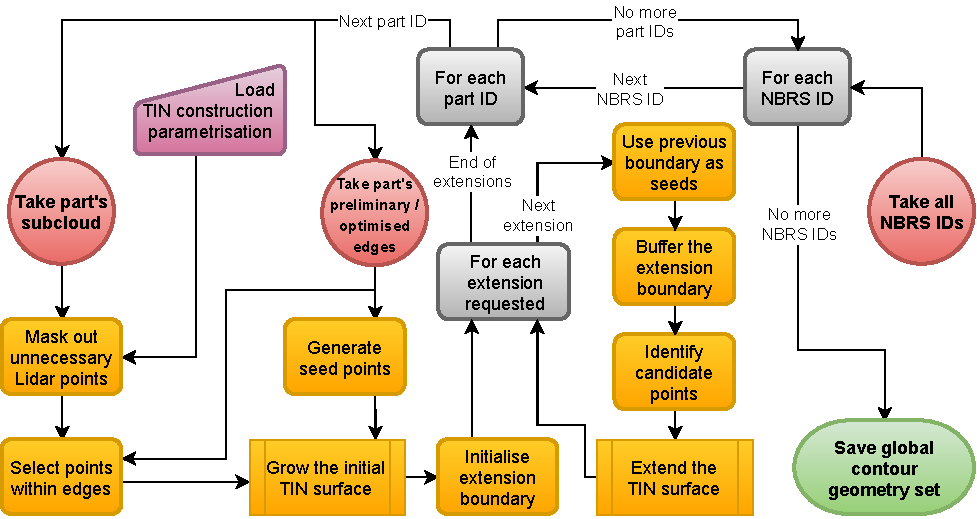
\includegraphics[width=\linewidth]{final_report/figs/tin_construction.pdf}
    \caption{Flowchart-style overview of the \ac{tin} construction step of the pipeline.}
    \label{fig:tinconstructionflow}
\end{figure}

\subsubsection{Preparation for \ac{tin} initialisation}

Based on the parametrisation, the outermost boundary within which points will be considered for insertion (including \ac{tin} extension) is constructed as a polygon, and points falling outside of its interior are excluded from further consideration. Then, either the preliminary edges or the optimised edges are fetched for the given \ac{nbrs} part. Since they are almost identical structurally, they can be treated the same way for the most part.

They are used for two tasks: firstly, to construct a line halfway between the two edges to form the basis of seeding the \ac{tin}, and secondly, to select points that fall within the edges as insertion candidates for the \ac{tin} initialisation step. This step is labelled \textit{"Grow the initial \ac{tin} surface"} in Figure \ref{fig:tinconstructionflow}, marked as a pre-defined procedure because the underlying procedure is fairly complex. To keep the complexity of the flowchart manageable, both the \ac{tin} initialisation and the \ac{tin} extension workflows of this step are illustrated in a separate diagram, shown in Figure \ref{fig:tinconstructiondetailsflow}.

\subsubsection{TIN initialisation}

\ac{tin} initialisation refers to the process of constructing an initial, conservative approximation of the road surface. As I noted above, it considers those Lidar points only, which fall between the preliminary or optimised edges. It first looks up those Lidar points, which are very close to the seed points. As these points are all but guaranteed to fall on the real-life road surface, they are unconditionally inserted into the \ac{tin} and are then pushed on a stack that in this case I will refer to as the "buffer". At this point in the algorithm, as Figure \ref{fig:tinconstructiondetailsflow} shows, we leave the \textit{"\ac{tin} initialisation"} group of operations and enter the \textit{"\ac{tin} growing"} group (which is shared with \textit{"\ac{tin} extension"}). The boundary vertices are also inserted into the \ac{tin} at this time (at an elevation of zero), which guarantees that the program can identify situations in which it is working with a triangle that is touching the boundary.

At this time, the \ac{tin} contains a high density of small triangles in the immediate vicinity of the original centreline of the \ac{nbrs} part. Furthermore, it contains large triangles connecting this area with the boundary inside of which the road surface is allowed to grow. During the initialisation stage, this boundary is represented by the preliminary edges or optimised edges themselves. Inserting these in the \ac{tin} serves a dual purpose. Firstly, it avoids raising errors when a conditional insertion test is being performed outside of the convex hull of inserted \ac{ahn3} and \ac{dtb} points. The boundary itself becomes the convex hull even before the insertions begin, so each time the program tries to locate the triangle into which a given point would be inserted, it will be guaranteed to succeed. Secondly, since the boundary is at an elevation of zero in the \ac{tin}, the program can easily identify when it is \textit{growing} the Lidar-defined surface because one or more of the located triangle's vertices will be found at an elevation of zero. This also means that the program is aware of the position of the tested points relative to the detailed surface and the boundary.

The buffer at this point consists of all the seed points that were inserted unconditionally. It is used to query all the points between the edges in a bulk KD-tree query, and is then emptied. All points returned by the query are pushed on a stack, and this stack forms the basis for the conditional insertions. One by one, the candidate points are popped, and are conditionally inserted into the \ac{tin}. Figure \ref{fig:tinconstructiondetailsflow} does not describe the conditions themselves, but I will go into detail about them here.

First, the triangle containing the popped point is located. If the triangle is defined only by subcloud points, then the elevation of the point according to the triangle is interpolated, and the difference in elevation is treated as an elevation discrepancy to which a threshold applies. If the threshold is not violated, then the distances to the three vertices of the triangle are computed, and based on that, the angles between the triangle's plane and the line segments connecting the popped point to the three vertices. If any of the three angles violate the applicable threshold, the point is not inserted.

If the located triangle contains one or more boundary points, the elevation discrepancy is computed in a different way. Growing the \ac{tin} needs to be done with some caution, as introducing erratic points around the edges of the current convex hull would entail that future insertions would have an incorrect basis for the conditional insertions and as a result, the surface would occasionally be allowed to grow in undesired directions. To minimise the chances of this happening, growing the surface takes into account multiple pre-existing \ac{tin} triangles in the neighbourhood, not just the closest ones. Specifically, all triangles containing the non-boundary vertices of the located triangle are fetched. Then, this is repeated with all the vertices of the resulting set of triangles. The vertices of this collection of nearby triangles are then fitted with a plane (re-using, once again, the least-squares method), and the distance of the tested point to the plane is taken to be a good approximation of the elevation discrepancy. Points in the buffer are always close to the pre-existing Lidar points in the \ac{tin} (see below for the reason), hence this is a reasonable assumption. The angle-based test is then administered the same way as for regular insertions.

Each popped point that ends up being inserted into the \ac{tin} is also pushed onto the buffer, which was previously emptied after it had been used for the KD-tree query to fill the stack. Once the stack becomes empty, the procedure restarts by performing another KD-tree query using the buffer, and refilling the stack with new points to try to insert. Only those points from the spatial query results are considered, which are not part of the \ac{tin} yet. In other words, as long as points are being inserted, and these points have \textit{uninserted} neighbours in the subcloud, the procedure will repeat. The buffer and the stack are kept separate so that KD-tree queries can be performed periodically as bulk operations, rather than individually - this is more efficient computationally.

As soon as no more insertions are taking place, the iteration ends and returns all points inserted into the \ac{tin}, in the order they were inserted. The \ac{tin} itself is not kept, instead it is reconstructed later on - this is due to the fact that point deletions in the triangulation package \textit{startin} do not appear to work reliably in this workflow, but we do not wish to keep the boundary points in the \ac{tin}. The straightforward way to achieve this without point removal is by reconstructing the \ac{tin} with the subcloud points only.

While the final implementation of this step is not too complex, it is in fact the result of an experimental development process in which several previous versions of the design were implemented and discarded after I found them lacking in effectiveness. The final version of the \ac{tin} initialisation procedure is effective, and not too complex computationally owing to the buffering-based implementation of the spatial queries. Other than improving its performance via adding the buffer-based approach, I also needed to improve its reliability. Originally, I implemented \ac{tin} point removals to remove the insertion boundaries. In fact, in the first version of the implementation, I inserted points and then conditionally \textit{removed} them depending on the geometry of the tree triangles created upon insertion. However, as I mentioned above, I found that using point removals in practice made \textit{startin} unstable, causing it to crash at random points in the process. However, from previous experience with this package, I knew that it is extremely efficient in building \ac{tin}s and interpolating in them, owing to its Rust-based implementation. Ultimately, I made to choice to keep using \textit{startin}, but to implement the workflow in a way that the \ac{tin}s are rebuilt once after initialisation (and then again after each extension iteration), "removing" the insertion boundaries implicitly.

A further important performance consideration was to efficiently find Lidar points falling within the insertion boundaries prior to starting the insertions. I found that testing the points one-by-one using \textit{shapely} takes an unacceptable toll on performance, hence I modified this procedure to work as a bulk task via the \codeword{path} module of \textit{matplotlib}, which is capable of finding points within a polygon formed of a single ring of coordinates with much lower computational complexity.

\begin{figure}
    \centering
    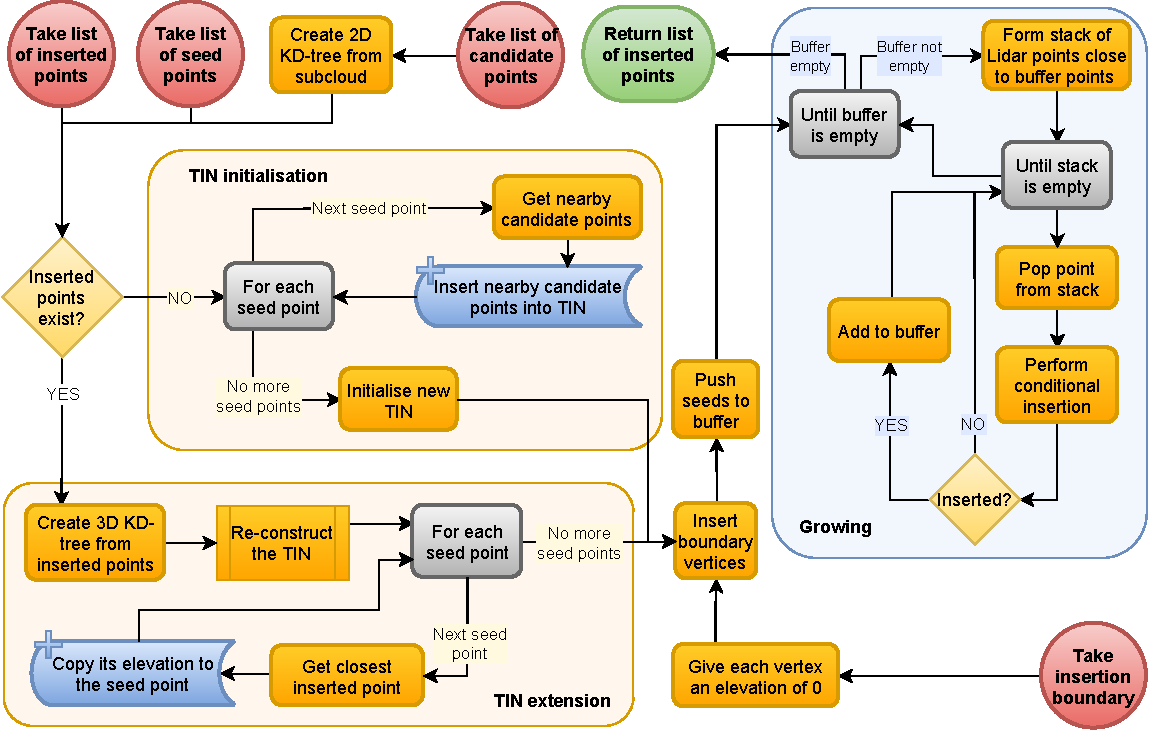
\includegraphics[width=\linewidth]{final_report/figs/tin_construction_details.pdf}
    \caption{Flowchart-style illustration of the details of \ac{tin} initialisation and construction.}
    \label{fig:tinconstructiondetailsflow}
\end{figure}

\subsubsection{TIN extension}

The extension of the \ac{tin} takes place in an iterative manner. The implementation accepts arguments that set the amount by which the boundary should be buffered in each iteration, as well as the number of extension iterations (steps). The starting boundary is \textit{not} the same as the one used during the initialisation of the \ac{tin}. There, the preliminary or optimised edges were used, but here the first iteration's boundary is buffered from the seed line (the line halfway between the preliminary or optimised edges). This allows the algorithm to take another look at the points between the edges in case in missed any good candidates during initialisation, while also allowing it to consider points outside the edges in later iterations.

The seeding of extension iterations is different than that of the initialisation step. The seed points are always derived from the boundary used in the previous iteration. Furthermore, in \ac{tin} initialisation the candidate points included all points between the road edges, whereas in the extension steps only the points located in-between the previous and the current boundary (in 2D), are considered. Depending on the parametrisation, the boundary may be buffered to examine areas \textit{beyond} the preliminary or optimised edges. This allows the program to try to grow the surface into areas which were not between the edges because of issues with the edges themselves. It is specifically intended to counteract the problem where road surfaces might get very thin where edge detection or optimisation significantly underestimated their width.

Each iteration first reconstructs the \ac{tin} yielded by the previous iteration, and inserts its new, buffered boundary into it. Since boundaries are always at an elevation of zero, when the previous iteration's boundary is reused to seed the current iteration, it first needs to be \textit{transposed to 3D}, otherwise spatial queries based on it would not work. This is done by creating a KD-tree from all pre-existing \ac{tin} vertices and associating the closest one's elevation with each vertex of the 2D geometry. It is then ready to seed the new iteration, by itself being the basis for KD-tree queries on the new candidate points. However, the results of this seed-query are not inserted into the \ac{tin} unconditionally like they are in \ac{tin} initialisation, because the assumption that points close to the seed geometry are sure to be part of the real-life road surface no longer holds. Instead, they are simply pushed to the buffer to start the main iteration involving the conditional insertions.

Once \ac{tin} extension has finished, the final \ac{tin} is reconstructed and is saved. Thus, one \ac{tin} object per \ac{nbrs} part is saved, and these are not merged or joined together into a single \ac{tin} in any way.

\subsubsection{Challenges encountered}

As implementing such a complex algorithm in this pipeline step was not originally intended, the biggest challenge here was to come up with a good solution within the timeframe reserved for the project. In terms of the methods themselves, I spent the most amount of time and effort on developing a solution that allows the road surface to grow into regions not covered by the preliminary or optimised edges. While in all cases, the surface generated by \ac{tin} initialisation is adequate to generate 3D-NWB, my desire was to not only model the central, traffic-occupied part of the road, but to grow it to the real-life edges of the paved surface as best as possible.

I initially wished to build the \ac{tin} as a single growing operation, but this proved to be prone to spreading into off-road regions. Depending on what order certain groups of points are examined in, even relatively sharp breaks in the underlying surface may appear smooth. A good way to deal with this problem would have been to decrease the query radius used in the buffer queries, but this in turn often prevented the \ac{tin} from growing at all. This is the reason why I eventually implemented the final version of the method as a combination of first initialising a conservative \ac{tin} in a large-scale growing operation, and then extending it carefully by examining thin "layers" of additional points progressing outwards from the centre of the road.

Performing conditional insertions outside of the convex hull of the pre-existing \ac{tin} points was also a challenge. Interpolating in the triangles is not a possibility here, but the importance of assessing the compliance of the tested points with the neighbourhood is ever so important - it depends on these surface growing insertions, whether a \ac{tin} might accidentally spread into an off-road area, or not.

\subsection{TIN-based interpolation and vertex snapping}
\label{sub:m_interpolation}

\subsubsection{Interpolation and origin tracking}

This is the last step in the pipeline, and its primary purpose is to use the \ac{tin}s generated in the previous step to enrich the source road network with the final elevations. As Figure \ref{fig:elevationinterpolationflow} shows, the first step in this procedure involves iterating through all \ac{nbrs} parts, and performing the interpolation step itself on each of their vertices.

An additional step takes place during this iteration. To make it possible to keep track of which elevations come from where exactly, the algorithm recognises triangles that have vertices that originate from \ac{dtb}. Before performing the interpolation, the triangle in which the interpolation will take place is fetched, and the origin of its vertices is examined. If any of them are from \ac{dtb}, then the origin of the triangle is deemed to be \ac{dtb} overall. For simplicity, the algorithm does not explicitly indicate what mixture of \ac{ahn3} and \ac{dtb} vertices were found in the triangle. These labels are used in the accuracy estimation step, primarily to advise the user which output elevations were affected by \ac{dtb}, and should therefore be treated with some skepticism. Please refer to Sections \ref{sub:dtb} and \ref{sec:r_comparison} for more information about this topic.

The implementation uses linear interpolation in the \ac{tin}s (also called TIN-linear interpolation). This is one of the simplest interpolation techniques available for \ac{tin}s, and it is also the one most widely studied among them in the literature I studied (see Section \ref{sec:lidaraccuracy}). It is particularly suitable to this research, because its error propagation formulae are readily available in the literature, and because an implementation of it forms part of the \textit{startin} package which I use to build the \ac{tin}s and interpolate in them. This interpolator uses the barycentric position of the point where interpolation is desired. The closer it is to one of the vertices of located triangle, the bigger the vertex's influence becomes on the interpolated elevation. If it is closer to the centre of the triangle, the influence of the vertices is more evenly distributed. The technique is governed by the formula

$z_{p} =
\begin{bmatrix}
x_{pt}\\
y_{pt}\\ 
1
\end{bmatrix} =
\begin{bmatrix}
 a_{0} & a_{1} & a_{2} \\
 b_{0} & b_{1} & b_{2} \\
 c_{0} & c_{1} & c_{2}  
\end{bmatrix}
\begin{bmatrix}
z_{0}\\
z_{1}\\ 
z_{2}
\end{bmatrix}$

where $x_{pt}$ and $y_{pt}$ denote the X and Y coordinates of the location of interpolation (inside the triangle), the matrix in terms of $a_{0}$ to $c_{2}$ contains terms dependent on the 2D geometry of the triangle, and where the last vector corresponds to the three elevations of the three vertices of the triangle. Lastly, $z_{p}$ is the interpolated elevation. Please refer to \cite{fan_etal_2014} for the expressions for $a_{0}$ to $c_{2}$.

\begin{figure}
    \centering
    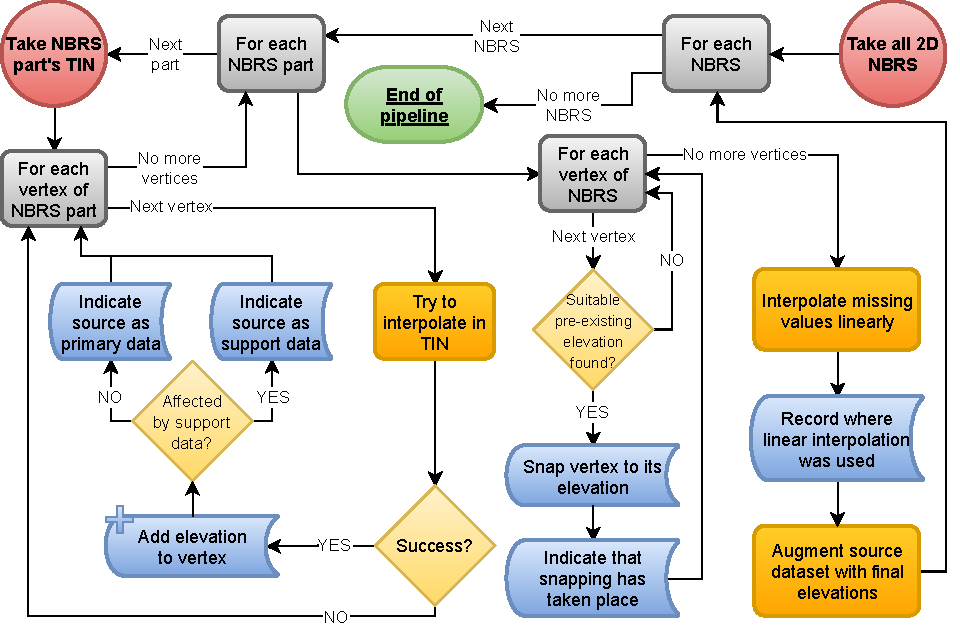
\includegraphics[width=\linewidth]{final_report/figs/elevation_interpolation.pdf}
    \caption{Flowchart-style illustration of the elevation interpolation step of the pipeline.}
    \label{fig:elevationinterpolationflow}
\end{figure}

\subsubsection{Vertex snapping and gap filling}

The next step is to perform vertex snapping at intersections. \ac{tin} surfaces close to intersections are expected to be comprised of roughly the same vertices, hence the assumption is made that snapping intersection vertices together will not introduce abrupt elevation discontinuities. The procedure, performed for each \ac{nbrs}, consists of taking each vertex one by one, and constructing a hashed data structure mapping their approximate 2D positions (coordinates to one decimal) to their exact elevations. In the underlying iteration, if the approximate 2D position of a point is already found to exist in the hashed storage, its elevation is replaced with the one already mapped to that 2D location (i.e. it is snapped to it). Since self-intersections of \ac{nbrs} are not possible, such a match necessarily represents a location where one or more other \ac{nbrs} end or begin - in other words, a real-life intersection.

Due to \ac{nwb}'s coarse georeferencing (often only one decimal or no decimals), checking 2D matches of coordinates is not enough. Each time a match is found, vertical distance is also examined prior to snapping, to avoid snapping together vertices that are at (nearly) perfectly matching 2D coordinates, but which in fact belong to roads that are in a non-intersecting 3D relationship, i.e. one passes above the other.

The last step of the procedure is to infill gaps in the elevation profiles left by failed interpolation. Missing elevations are most commonly the result of there not being \ac{ahn3} and \ac{dtb} coverage in a certain place. Vertices in such locations are not part of an \ac{nbrs} part, meaning that their elevations cannot be extracted from an underlying \ac{tin}. Elevations may also occasionally be missing due to problems with the preliminary or optimised edges, in turn mostly due to the problems with \ac{nwb}'s georeferencing.

These gaps are filled in using linear interpolation, and instead of indicating their origin as either \ac{ahn3} or \ac{dtb}, it is recorded to be the result of such interpolation.

\subsubsection{Outputting 3D-NWB}

The last step of the pipeline converts the internal road centreline data structure of the program (\ac{nbrs} parts and \ac{nbrs}) back into the data structure used by the input data, which are the LineStrings that are called \textit{wegvakken} in \ac{nwb}. In effect, the 2D geometry of each input LineString is overwritten with the new 3D geometry created using the original 2D coordinates, and the newly generated final elevations. Unlike at the end of preliminary elevation estimation (see Section \ref{sub:m_elevationestimation}), the original orientations of the \textit{wegvakken} is automatically respected irrespective of some of them having been internally flipped earlier in the pipeline. This is because the elevations are taken from the hashed data structures linking 2D positions to elevations, not from the flipped internal representations of these geometries.

\subsubsection{Challenges encountered}

As the tasks carried out in this pipeline step are relatively trivial, all challenges encountered were equally simple to solve. The only part of the implementation that proved to be less straightforward was the tracking of the origin of vertices through the \ac{tin}-based interpolation - this required some minor modifications to previous steps. The implemented approach is based on hashing: all \ac{dtb} points that make it into the subcloud of an \ac{nbrs} part are stored in a hashed data structure at one decimal precision of their coordinates, making it quick to identify whether one of the triangle's vertices are among them that is being used for the interpolation of an \ac{nwb} vertex.

\section{Accuracy assessment}
\label{sec:m_accuracyassessment}

As I explained in Section \ref{sub:accuracyoverview}, the estimation of output accuracy assumes no other influences than that which can be propagated through the interpolation technique relative to the input accuracy, in zones that are properly sampled. Identifying such regions and computing output accuracy represent the two main tasks in this step, the details of which are explained in this section.

\subsection{Detecting regions with poor sampling}
\label{sub:m_accuracypoorsampling}

\subsubsection{Details of sampling-related assumption}

The circumstance that local sampling density \textit{below a threshold value} does not affect interpolation accuracy is proven by previous work in this field, as mentioned in my literature review results. Of particular importance for us is \cite{guo_etal_2010}, which provides the most amount of detail on this topic. Neither this work, nor any other work to my knowledge derives an explicit mathematical formula that expresses a relationship between local sampling density and output accuracy below the threshold level, but this is not strictly necessary for my research, for a specific reason which I outline below.

\ac{ahn3} has a nominal mean point posting distance of around 30 to 40 centimetres (6 to 10 points per m\textsuperscript{2}). Considering that the dataset has a high vertical and horizontal accuracy (around 15 to 20 centimetres at two standard deviations), we may start to suspect that \ac{tin}s generated directly from \ac{ahn3} will heavily oversample the road surfaces. Any unevenness seen in the models will be due to stochastic Lidar \textit{noise}, rather than systematic errors due to local variations in sampling density or real-life road features.

In practice, the sampling density on road surfaces is often even higher than the nominal value I quoted above (see Section \ref{sec:accuracy}). At such exceptionally high baseline sampling rates, typical small-scale variations in local sampling density are of no consequence regarding the overall output accuracy. This is simply because these random, stochastic variations will never decrease the local point density to anywhere near the threshold below which output accuracy would become affected.

\subsubsection{Picking an appropriate threshold}

The thresholds I used are based on the results of \cite{guo_etal_2010}. They concluded that in the case of general terrain (not roads specifically) modelled by a raster \ac{dtm} at a 0.5 m resolution, \ac{rmse} with respect to control points does not significantly decrease below 0.2 points per grid cell. Cross-validation-based \ac{rmse} values around this density were still consistently below 20 cm. In other words, 0.2 points per 0.25 m\textsuperscript{2} appears to be sufficient, or equivalently, 0.8 points per 1 m\textsuperscript{2}. This is much lower than \ac{ahn3}'s mean density of 6 to 10 points per 1 m\textsuperscript{2}, especially considering that this is even higher on locally on road surfaces owing to their flatness. Furthermore, the Lidar data used in \cite{guo_etal_2010} has inferior accuracy relative to \ac{ahn3}.

The extra points may be useful for detecting small-scale features (such as e.g. small slumps in the roads surface), as well as better characterising the edges of roads. However, if we look at the problem strictly from the point of view of the 3D conversion of \ac{nwb} and the modelling of the surface's overall shape, then we are only interested in monitoring where the point density goes below the threshold above which the \ac{rmse} with respect to surveyed control points remains relatively constant. If we assume that about 1 point per 1 m\textsuperscript{2} is sufficient to characterise a rugged surface using Lidar, then we could consider drops of up to 95\% in \ac{ahn3}'s point density to be acceptable.

To make sure I use a conservative value, I opted to stay somewhat above this estimate. At each \ac{nwb} vertex, I examine the number of \ac{tin} vertices that fall within 3 metres of it, and if it is less than 3 points, then flag the output accuracy at that point to be unreliable. This corresponds to a a threshold of 3 points per 1 m\textsuperscript{2}.

\subsubsection{Types of areas violating the assumption}

In most places, the local sampling density must drop by more than 80\% to reach the above minimum threshold, which means that it only happens in extreme events. As we lack a mathematical formulation describing the exact nature of the influence below the threshold sampling rate, the best we can do is mark the accuracy of vertices falling into such areas as \textit{unknown} in the output.

Places where linear interpolation was used, the threshold-based evaluation is automatically assumed to be violated. They generally correspond to areas where there is no \ac{ahn3} and \ac{dtb} coverage, meaning that the local sampling density is zero, or nearly zero. Even in areas where linear interpolation had to be used due to the poor georeferencing of \ac{nwb}, the values were not based on the samples in the local \ac{tin}s, hence sampling density can considered to be zero there, too.

The threshold may also be violated due to an insufficient amount of detail in the \ac{tin}, but this is atypical in practice. Sampling density can only reach such low values in the \ac{tin}s due to \textit{significant} amounts of occlusion due to objects opaque to Lidar (so not vegetation). Notably, the threshold of 3 points per m\textsuperscript{2} deems it reasonable to regard most elevations reliable which were interpolated inside medium-sized gaps resulting from vehicles or other stationary objects on the roads, as well as some that are found in regions where only \ac{dtb} coverage is available - although the latter should be treated with some skepticism, as I noted in Section \ref{sub:accuracyoverview} earlier in this chapter.

\subsection{Effect of interpolation of accuracy}
\label{sub:m_accuracyinterpolation}

Theoretical proof suggests that the interpolation step generally \textit{improves}, rather than deteriorates the output accuracy. This can intuitively be thought of as the result of basing each output elevation on the combined information stored in the three vertices of the triangle in which the elevation is being interpolated.

This is contrary to what one might assume based on thinking about the pipeline as a whole, but both in practice and in theory, it is the \textit{other} influences on accuracy that generally have the opposite effect. For instance, problems with ground filtering and a sparse local sampling may have negative effects on accuracy locally. However, the interpolation itself has no such effect on the output under normal circumstances. We can thus assert that the formal accuracy of the output will \textit{mostly} increase relative to the input in well-sampled regions. I present the relevant error propagation results from \cite{fan_etal_2014} below.

Let $\sigma_{z_{vx}}^{2}$ denote the elevation variance of the vertices of the triangle, and $\sigma_{xy_{vx}}^{2}$ denote the horizontal variance. We may then express the relationship between the elevation accuracy at the point of interpolation $\sigma_{z_{pt}}^{2}$ as

$\sigma_{z_{pt}}^{2} = M\left(\sigma_{z_{vx}}^{2} + \sigma_{z_{node}}^{2}\left(tan\left(\alpha_x\right)^2 + tan\left(\alpha_y\right)^2\right)\right)$

where $tan\left(\alpha_x\right)^2$ and $tan\left(\alpha_y\right)^2$ correspond to the angle between the triangle's plane and the X and Y axes of the CRS. The expression takes into account the steepness of the plane to be able to propagate the horizontal error, hence the necessity of computing these angles. The variable $M$ is a parameter that needs to be pre-computed for each triangle, as it depends on their 3D geometry. The underlying formula will not be listed here as it is not relevant to this discussion, please refer to the original paper for it.

Since \ac{ahn3} and \ac{dtb} points and vertices have no individual accuracy measurements, the above formula takes a single accuracy value per triangle, rather than a separate value for each vertex. Like in the origin-labelling step I described in Section \ref{sub:m_interpolation}, I make the assumption that \ac{dtb}'s accuracy should only be used in this formula, if all three triangle vertices are based on \ac{dtb} data.

The expression is, in essence, a sum of the input variances scaled by geometric variables. Most importantly $M$ has a range between about 1/3 and 1, taking its lowest value around the centroid of the triangle, and increasing to 1 at the triangle's vertices. Intuitively, the closer we are interpolating to one of the vertices, the smaller the other two vertices' influence is going to be due to the nature of TIN-linear interpolation. We are thereby gradually taking into account less and less information, decreasing to the minimum at the vertices, where only one input elevation measurement is considered. Assuming that the \ac{nwb} vertices are randomly distributed relative to triangle vertices, the expected value of $M$ is 0.5.

Substituting values into the above formula with $M=0.5$ reveals that applying TIN-linear interpolation to surfaces with sufficiently low inclinations decreases the elevation error relative to the input. For instance, a triangle with a 2-degree inclination and vertices with 10 cm vertical and horizontal standard deviations (similar to \ac{ahn3}) yields an output elevation standard deviation of 7 cm, a 30\% decrease. Increasing the inclination to 45 degrees decreases the vertical accuracy of the output to 12 cm, which is now worse than that of the input.

Such steep roads are practically absent in The Netherlands. For Dutch roads, the accuracy is thus expected to increase. However, oversampling the surfaces too heavily with a non-zero stochastic scatter in the elevations can yield small artefact triangles that are inclined anomalously. These inclinations are meaningless, as they do not represent the geometry of the underlying road surfaces, and care should thus be exercised when interpreting the accuracy assessment values of results that were generated using most of the original Lidar points. More information on this topic is found in Section \ref{sec:accuracy}.

\subsection{Evaluating TIN surface completeness}
\label{sub:m_accuracycompleteness}

To evaluate how complete the generated \ac{tin} road surfaces are relative to the true road surfaces, I relied on a visual comparison of the \ac{tin}s with the subclouds, as well as on a comparison with \ac{bgt} (\cite{bgt_homepage}). Like \ac{ahn3} and \ac{dtb}, it is a Dutch open data geospatial dataset. It is maintained by Kadaster, the national cadastral agency. It is a topographical map of the country which contains a wide range of classified areal features - such as city, building, and \textit{road} extents.

Like \ac{nwb}, \ac{bgt} is also primarily intended to offer good topological accuracy, thus its 2D georeferencing is also relatively crude. However, upon a comparison with the Luchtfoto 2020 orthoimagery (also from Kadaster, see \cite{luchtfoto_pdok}), I deemed its road polygons reliable and accurate enough to serve as a reference with which my results can be compared. To make the comparison, I plotted some of the output \ac{tin}s against the relevant \ac{bgt} road outlines in 2D and assessed the agreement between them visually. An example of the results of this step, as well as a comparison of \ac{bgt} and \ac{nwb} with satellite imagery, are shown in Figure \ref{fig:bgtcomparison}.

\section{Comparison with commercial results}
\label{sec:m_comparison}

A simple method to evaluate the relative quality and accuracy of the commercial results is to examine variations in the agreement between the elevations predicted by the academic and commercial results visually, and quantitatively by computing residuals and \ac{rmse} values.

However, we know from the previous section that the academic results have an output accuracy that is either on par with or better than that of the input, with the exception of areas with poor sampling density. Where the sampling density is high, we can use the academic results as reference to advise us about the \textit{absolute} accuracy of the commercial results, not just relative to the academic ones.

In places where the academic results have unknown accuracy, the commercial elevations are also necessarily uncertain because the same datasets were used in their production. However, their overall quality may still be different than ours, because their methods use the input data differently. In such places, the comparison relies on human interpretation. To aid the interpretation, I computed and plotted the residuals between the two sets of results in a number of LineStrings (\textit{wegvakken}) that I picked for comparison. Correlating these with comparison plots of the elevation series, as well as 3D plots of the data and underlying \ac{ahn3} and \ac{dtb} points provided further input to this process. I also employed the generation of \ac{rmse} values on the level of \textit{wegvakken}, as well as for entire testing datasets. The \ac{rmse} is given by

$RMSE = \sqrt{\frac{\sum_{t=1}^{T}\left(z_{a,t} - z_{c,t}\right)^2}{T}}$

where the elevation samples in a profile are numbered from $t=1$ to $T$, and where $z_{c,t}$ denotes the elevation estimated by my method and $z_{c,t}$ denotes the commercial result at the same location.

When performing the above comparison on a LineString, the distances from its first vertex along the profile from $t=1$ to $T$ are computed, this is what the elevation series and residuals are plotted against. The residuals are the values taken by $z_{a,t_{nwb}} - z_{c,t_{nwb}}$ where $t_{nwb}$ corresponds to \textit{original \ac{nwb} vertices}. Both the academic and the commercial pipelines use vertex densification, but the resulting vertices are not located in the same place. Thus, the residuals and the \ac{rmse} values describe only how well the two methods agree at the location of the \textit{original} \ac{nwb} vertices.

\section{Programming framework}
\label{sec:programming}

The implementation part of this project is intended to investigate how well each step of the pipeline works in practice, how well they work together as a pipeline, and how accurate their output is. In turn, these serve the purpose of answering the research questions detailed in Section \ref{sec:rq}. In addition, implementation-related tasks were also important in iteratively revising the methods based on the practical experience gained in the process, making them better adapted to real-life scenarios (and as result, more relevant to reusers).

\subsubsection{Notes on performance}

As the implementation is primarily intended for demonstration and reference purposes, it is by no means ready for all types of academic and commercial use out of the box. One limiting factor in this sense is the lack of a scaling mechanism in the implementation, as such considerations were not part of this research. Furthermore, I developed all parts of the pipeline in Python 3.8, which means that the code is more concise than a binary implementation would be, but its runtimes are higher. To improve performance, I relied on binary-based libraries such as \textit{numpy}, and parts of \textit{scipy}. In addition, I used hashing-based data structures (in Python these are called dictionaries and sets) extensively, which are also known to benefit performance greatly. Many of these uses of hashing are mentioned previous sections explicitly, and wherever I mention using KD-trees, I refer to building code on top of the binary implementation in \textit{scipy}. Uses of \textit{numpy} are so pervasive in the code, that I opted not to mention them explicitly in the text.

While geometries (and geometric operations) are often handled in \textit{shapely}, I avoided its use in all cases where geometries are bulk-processed via long iterations. I found that implementing the geometric operations from first principles in \textit{numpy} in such cases resulted in a noticeable gain in performance.

Unfortunately, the implementation of active contour optimisation in \textit{scikit-image} is mostly based on native Python iterations, not on binary packages. This circumstance, in conjunction with the large number of vector inner products that the attractor map generation requires, means that the computational complexity of the active contour-related part of my software is a magnitude slower than all other parts.

\subsubsection{GitHub release and code structure}

I released the source code of the implementation in the following GitHub repository:
\url{https://github.com/kriskenesei/geo2020-modules}. Most functionality resides in the class \codeword{nbrs_manager} inside the file \codeword{nbrs_generation.py}. I factored out some functionality into \codeword{lib_shared.py} to somewhat simplify the code in \codeword{nbrs_generation.py}. Both files contain an extensive set of docstrings and inline guidance on what each part of the code does. The intended audience of this information includes those simply interested in knowing more about the practical aspects of processing that underlies this research, as well as potential reusers.

The class \codeword{nbrs_manager} is intended to be instantiated with the cropped road network, followed by the invocation of class methods corresponding to each pipeline step. In addition, vertex densification is also implemented as its own class method, and a range of methods are provided for basic operations such as setting individual \textit{wegvak} geometry, as well as writing the intermediate results of each pipeline step to disk separately. Furthermore, the class holds certain intermediate results in its class variables which cannot be written to disk natively, but which may be interesting to reusers.

The structure of relevant part of the next chapter (Section \ref{sec:results}) is modelled on the steps one would take to run my software, to create a stronger link between the explanations and the implementation. The method invocations that I used to generate the results shown in the chapter are explicitly listed at the end of the sections describing the relevant pipeline steps. A condensed explanation of how the implementation is meant to be used can also be found in the docstring of \codeword{nbrs_manager}, and a set of example calls are also provided at the end of the file \codeword{nbrs_generation.py}.